% Options for packages loaded elsewhere
\PassOptionsToPackage{unicode}{hyperref}
\PassOptionsToPackage{hyphens}{url}
%
\documentclass[
]{book}
\usepackage{amsmath,amssymb}
\usepackage{iftex}
\ifPDFTeX
  \usepackage[T1]{fontenc}
  \usepackage[utf8]{inputenc}
  \usepackage{textcomp} % provide euro and other symbols
\else % if luatex or xetex
  \usepackage{unicode-math} % this also loads fontspec
  \defaultfontfeatures{Scale=MatchLowercase}
  \defaultfontfeatures[\rmfamily]{Ligatures=TeX,Scale=1}
\fi
\usepackage{lmodern}
\ifPDFTeX\else
  % xetex/luatex font selection
\fi
% Use upquote if available, for straight quotes in verbatim environments
\IfFileExists{upquote.sty}{\usepackage{upquote}}{}
\IfFileExists{microtype.sty}{% use microtype if available
  \usepackage[]{microtype}
  \UseMicrotypeSet[protrusion]{basicmath} % disable protrusion for tt fonts
}{}
\makeatletter
\@ifundefined{KOMAClassName}{% if non-KOMA class
  \IfFileExists{parskip.sty}{%
    \usepackage{parskip}
  }{% else
    \setlength{\parindent}{0pt}
    \setlength{\parskip}{6pt plus 2pt minus 1pt}}
}{% if KOMA class
  \KOMAoptions{parskip=half}}
\makeatother
\usepackage{xcolor}
\usepackage{color}
\usepackage{fancyvrb}
\newcommand{\VerbBar}{|}
\newcommand{\VERB}{\Verb[commandchars=\\\{\}]}
\DefineVerbatimEnvironment{Highlighting}{Verbatim}{commandchars=\\\{\}}
% Add ',fontsize=\small' for more characters per line
\usepackage{framed}
\definecolor{shadecolor}{RGB}{248,248,248}
\newenvironment{Shaded}{\begin{snugshade}}{\end{snugshade}}
\newcommand{\AlertTok}[1]{\textcolor[rgb]{0.94,0.16,0.16}{#1}}
\newcommand{\AnnotationTok}[1]{\textcolor[rgb]{0.56,0.35,0.01}{\textbf{\textit{#1}}}}
\newcommand{\AttributeTok}[1]{\textcolor[rgb]{0.13,0.29,0.53}{#1}}
\newcommand{\BaseNTok}[1]{\textcolor[rgb]{0.00,0.00,0.81}{#1}}
\newcommand{\BuiltInTok}[1]{#1}
\newcommand{\CharTok}[1]{\textcolor[rgb]{0.31,0.60,0.02}{#1}}
\newcommand{\CommentTok}[1]{\textcolor[rgb]{0.56,0.35,0.01}{\textit{#1}}}
\newcommand{\CommentVarTok}[1]{\textcolor[rgb]{0.56,0.35,0.01}{\textbf{\textit{#1}}}}
\newcommand{\ConstantTok}[1]{\textcolor[rgb]{0.56,0.35,0.01}{#1}}
\newcommand{\ControlFlowTok}[1]{\textcolor[rgb]{0.13,0.29,0.53}{\textbf{#1}}}
\newcommand{\DataTypeTok}[1]{\textcolor[rgb]{0.13,0.29,0.53}{#1}}
\newcommand{\DecValTok}[1]{\textcolor[rgb]{0.00,0.00,0.81}{#1}}
\newcommand{\DocumentationTok}[1]{\textcolor[rgb]{0.56,0.35,0.01}{\textbf{\textit{#1}}}}
\newcommand{\ErrorTok}[1]{\textcolor[rgb]{0.64,0.00,0.00}{\textbf{#1}}}
\newcommand{\ExtensionTok}[1]{#1}
\newcommand{\FloatTok}[1]{\textcolor[rgb]{0.00,0.00,0.81}{#1}}
\newcommand{\FunctionTok}[1]{\textcolor[rgb]{0.13,0.29,0.53}{\textbf{#1}}}
\newcommand{\ImportTok}[1]{#1}
\newcommand{\InformationTok}[1]{\textcolor[rgb]{0.56,0.35,0.01}{\textbf{\textit{#1}}}}
\newcommand{\KeywordTok}[1]{\textcolor[rgb]{0.13,0.29,0.53}{\textbf{#1}}}
\newcommand{\NormalTok}[1]{#1}
\newcommand{\OperatorTok}[1]{\textcolor[rgb]{0.81,0.36,0.00}{\textbf{#1}}}
\newcommand{\OtherTok}[1]{\textcolor[rgb]{0.56,0.35,0.01}{#1}}
\newcommand{\PreprocessorTok}[1]{\textcolor[rgb]{0.56,0.35,0.01}{\textit{#1}}}
\newcommand{\RegionMarkerTok}[1]{#1}
\newcommand{\SpecialCharTok}[1]{\textcolor[rgb]{0.81,0.36,0.00}{\textbf{#1}}}
\newcommand{\SpecialStringTok}[1]{\textcolor[rgb]{0.31,0.60,0.02}{#1}}
\newcommand{\StringTok}[1]{\textcolor[rgb]{0.31,0.60,0.02}{#1}}
\newcommand{\VariableTok}[1]{\textcolor[rgb]{0.00,0.00,0.00}{#1}}
\newcommand{\VerbatimStringTok}[1]{\textcolor[rgb]{0.31,0.60,0.02}{#1}}
\newcommand{\WarningTok}[1]{\textcolor[rgb]{0.56,0.35,0.01}{\textbf{\textit{#1}}}}
\usepackage{longtable,booktabs,array}
\usepackage{calc} % for calculating minipage widths
% Correct order of tables after \paragraph or \subparagraph
\usepackage{etoolbox}
\makeatletter
\patchcmd\longtable{\par}{\if@noskipsec\mbox{}\fi\par}{}{}
\makeatother
% Allow footnotes in longtable head/foot
\IfFileExists{footnotehyper.sty}{\usepackage{footnotehyper}}{\usepackage{footnote}}
\makesavenoteenv{longtable}
\usepackage{graphicx}
\makeatletter
\def\maxwidth{\ifdim\Gin@nat@width>\linewidth\linewidth\else\Gin@nat@width\fi}
\def\maxheight{\ifdim\Gin@nat@height>\textheight\textheight\else\Gin@nat@height\fi}
\makeatother
% Scale images if necessary, so that they will not overflow the page
% margins by default, and it is still possible to overwrite the defaults
% using explicit options in \includegraphics[width, height, ...]{}
\setkeys{Gin}{width=\maxwidth,height=\maxheight,keepaspectratio}
% Set default figure placement to htbp
\makeatletter
\def\fps@figure{htbp}
\makeatother
\setlength{\emergencystretch}{3em} % prevent overfull lines
\providecommand{\tightlist}{%
  \setlength{\itemsep}{0pt}\setlength{\parskip}{0pt}}
\setcounter{secnumdepth}{5}
\usepackage{booktabs}
\ifLuaTeX
  \usepackage{selnolig}  % disable illegal ligatures
\fi
\usepackage[]{natbib}
\bibliographystyle{plainnat}
\usepackage{bookmark}
\IfFileExists{xurl.sty}{\usepackage{xurl}}{} % add URL line breaks if available
\urlstyle{same}
\hypersetup{
  pdftitle={Theory-driven analysis of ecological data: a practical handbook},
  pdfauthor={us},
  hidelinks,
  pdfcreator={LaTeX via pandoc}}

\title{Theory-driven analysis of ecological data: a practical handbook}
\author{us}
\date{2024-11-22}

\usepackage{amsthm}
\newtheorem{theorem}{Theorem}[chapter]
\newtheorem{lemma}{Lemma}[chapter]
\newtheorem{corollary}{Corollary}[chapter]
\newtheorem{proposition}{Proposition}[chapter]
\newtheorem{conjecture}{Conjecture}[chapter]
\theoremstyle{definition}
\newtheorem{definition}{Definition}[chapter]
\theoremstyle{definition}
\newtheorem{example}{Example}[chapter]
\theoremstyle{definition}
\newtheorem{exercise}{Exercise}[chapter]
\theoremstyle{definition}
\newtheorem{hypothesis}{Hypothesis}[chapter]
\theoremstyle{remark}
\newtheorem*{remark}{Remark}
\newtheorem*{solution}{Solution}
\begin{document}
\maketitle

{
\setcounter{tocdepth}{1}
\tableofcontents
}
\chapter{About Bookdown}\label{about-bookdown}

This is a \emph{sample} book written in \textbf{Markdown}. You can use anything that Pandoc's Markdown supports; for example, a math equation \(a^2 + b^2 = c^2\).

\section{Usage}\label{usage}

Each \textbf{bookdown} chapter is an .Rmd file, and each .Rmd file can contain one (and only one) chapter. A chapter \emph{must} start with a first-level heading: \texttt{\#\ A\ good\ chapter}, and can contain one (and only one) first-level heading.

Use second-level and higher headings within chapters like: \texttt{\#\#\ A\ short\ section} or \texttt{\#\#\#\ An\ even\ shorter\ section}.

The \texttt{index.Rmd} file is required, and is also your first book chapter. It will be the homepage when you render the book.

\section{Render book}\label{render-book}

You can render the HTML version of this example book without changing anything:

\begin{enumerate}
\def\labelenumi{\arabic{enumi}.}
\item
  Find the \textbf{Build} pane in the RStudio IDE, and
\item
  Click on \textbf{Build Book}, then select your output format, or select ``All formats'' if you'd like to use multiple formats from the same book source files.
\end{enumerate}

Or build the book from the R console:

\begin{Shaded}
\begin{Highlighting}[]
\NormalTok{bookdown}\SpecialCharTok{::}\FunctionTok{render\_book}\NormalTok{()}
\end{Highlighting}
\end{Shaded}

To render this example to PDF as a \texttt{bookdown::pdf\_book}, you'll need to install XeLaTeX. You are recommended to install TinyTeX (which includes XeLaTeX): \url{https://yihui.org/tinytex/}.

\section{Preview book}\label{preview-book}

As you work, you may start a local server to live preview this HTML book. This preview will update as you edit the book when you save individual .Rmd files. You can start the server in a work session by using the RStudio add-in ``Preview book'', or from the R console:

\begin{Shaded}
\begin{Highlighting}[]
\NormalTok{bookdown}\SpecialCharTok{::}\FunctionTok{serve\_book}\NormalTok{()}
\end{Highlighting}
\end{Shaded}

\section{Here are some useful things for writing the book using bookdown}\label{here-are-some-useful-things-for-writing-the-book-using-bookdown}

All chapters start with a first-level heading followed by your chapter title, like the line above. There should be only one first-level heading (\texttt{\#}) per .Rmd file.

\subsection{A section}\label{a-section}

All chapter sections start with a second-level (\texttt{\#\#}) or higher heading followed by your section title, like the sections above and below here. You can have as many as you want within a chapter.

\subsubsection*{An unnumbered section}\label{an-unnumbered-section}
\addcontentsline{toc}{subsubsection}{An unnumbered section}

Chapters and sections are numbered by default. To un-number a heading, add a \texttt{\{.unnumbered\}} or the shorter \texttt{\{-\}} at the end of the heading, like in this section.

\section{Cross-references}\label{cross}

Cross-references make it easier for your readers to find and link to elements in your book.

\subsection{Chapters and sub-chapters}\label{chapters-and-sub-chapters}

There are two steps to cross-reference any heading:

\begin{enumerate}
\def\labelenumi{\arabic{enumi}.}
\tightlist
\item
  Label the heading: \texttt{\#\ Hello\ world\ \{\#nice-label\}}.

  \begin{itemize}
  \tightlist
  \item
    Leave the label off if you like the automated heading generated based on your heading title: for example, \texttt{\#\ Hello\ world} = \texttt{\#\ Hello\ world\ \{\#hello-world\}}.
  \item
    To label an un-numbered heading, use: \texttt{\#\ Hello\ world\ \{-\#nice-label\}} or \texttt{\{\#\ Hello\ world\ .unnumbered\}}.
  \end{itemize}
\item
  Next, reference the labeled heading anywhere in the text using \texttt{\textbackslash{}@ref(nice-label)}; for example, please see Chapter \ref{cross}.

  \begin{itemize}
  \tightlist
  \item
    If you prefer text as the link instead of a numbered reference use: \hyperref[cross]{any text you want can go here}.
  \end{itemize}
\end{enumerate}

\subsection{Captioned figures and tables}\label{captioned-figures-and-tables}

Figures and tables \emph{with captions} can also be cross-referenced from elsewhere in your book using \texttt{\textbackslash{}@ref(fig:chunk-label)} and \texttt{\textbackslash{}@ref(tab:chunk-label)}, respectively.

See Figure \ref{fig:nice-fig}.

\begin{Shaded}
\begin{Highlighting}[]
\FunctionTok{par}\NormalTok{(}\AttributeTok{mar =} \FunctionTok{c}\NormalTok{(}\DecValTok{4}\NormalTok{, }\DecValTok{4}\NormalTok{, .}\DecValTok{1}\NormalTok{, .}\DecValTok{1}\NormalTok{))}
\FunctionTok{plot}\NormalTok{(pressure, }\AttributeTok{type =} \StringTok{\textquotesingle{}b\textquotesingle{}}\NormalTok{, }\AttributeTok{pch =} \DecValTok{19}\NormalTok{)}
\end{Highlighting}
\end{Shaded}

\begin{figure}

{\centering 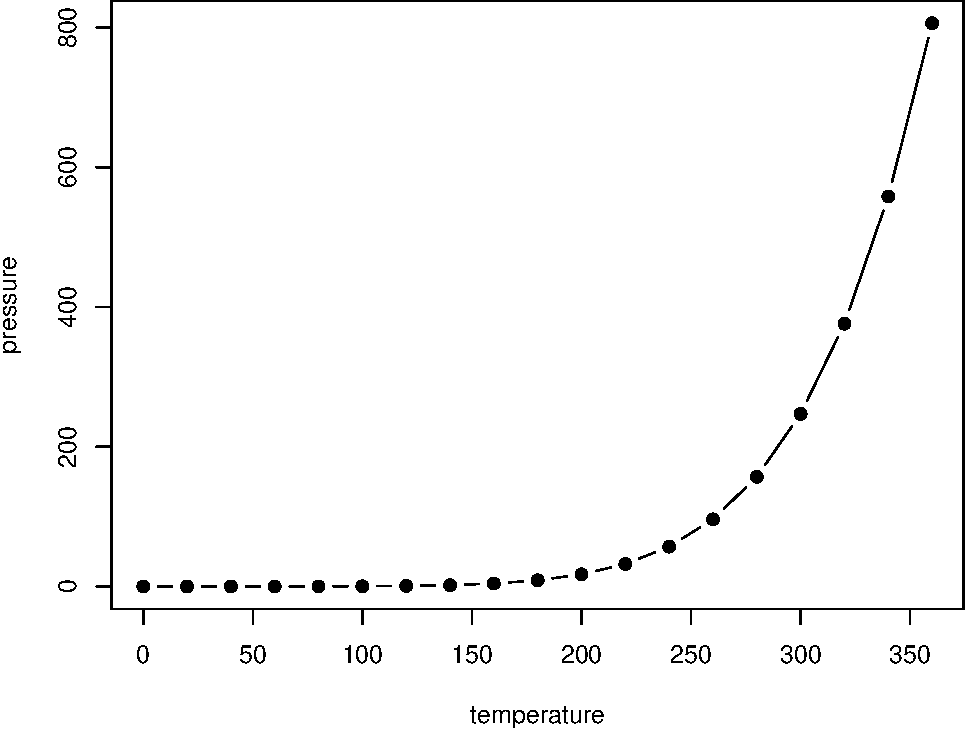
\includegraphics[width=0.8\linewidth]{_main_files/figure-latex/nice-fig-1} 

}

\caption{Here is a nice figure!}\label{fig:nice-fig}
\end{figure}

Don't miss Table \ref{tab:nice-tab}.

\begin{Shaded}
\begin{Highlighting}[]
\NormalTok{knitr}\SpecialCharTok{::}\FunctionTok{kable}\NormalTok{(}
  \FunctionTok{head}\NormalTok{(pressure, }\DecValTok{10}\NormalTok{), }\AttributeTok{caption =} \StringTok{\textquotesingle{}Here is a nice table!\textquotesingle{}}\NormalTok{,}
  \AttributeTok{booktabs =} \ConstantTok{TRUE}
\NormalTok{)}
\end{Highlighting}
\end{Shaded}

\begin{table}

\caption{\label{tab:nice-tab}Here is a nice table!}
\centering
\begin{tabular}[t]{rr}
\toprule
temperature & pressure\\
\midrule
0 & 0.0002\\
20 & 0.0012\\
40 & 0.0060\\
60 & 0.0300\\
80 & 0.0900\\
\addlinespace
100 & 0.2700\\
120 & 0.7500\\
140 & 1.8500\\
160 & 4.2000\\
180 & 8.8000\\
\bottomrule
\end{tabular}
\end{table}

\section{Parts}\label{parts}

You can add parts to organize one or more book chapters together. Parts can be inserted at the top of an .Rmd file, before the first-level chapter heading in that same file.

Add a numbered part: \texttt{\#\ (PART)\ Act\ one\ \{-\}} (followed by \texttt{\#\ A\ chapter})

Add an unnumbered part: \texttt{\#\ (PART\textbackslash{}*)\ Act\ one\ \{-\}} (followed by \texttt{\#\ A\ chapter})

Add an appendix as a special kind of un-numbered part: \texttt{\#\ (APPENDIX)\ Other\ stuff\ \{-\}} (followed by \texttt{\#\ A\ chapter}). Chapters in an appendix are prepended with letters instead of numbers.

\section{Footnotes and citations}\label{footnotes-and-citations}

\subsection{Footnotes}\label{footnotes}

Footnotes are put inside the square brackets after a caret \texttt{\^{}{[}{]}}. Like this one \footnote{This is a footnote.}.

\subsection{Citations}\label{citations}

Reference items in your bibliography file(s) using \texttt{@key}.

For example, we are using the \textbf{bookdown} package \citep{R-bookdown} (check out the last code chunk in index.Rmd to see how this citation key was added) in this sample book, which was built on top of R Markdown and \textbf{knitr} \citep{xie2015} (this citation was added manually in an external file book.bib).
Note that the \texttt{.bib} files need to be listed in the index.Rmd with the YAML \texttt{bibliography} key.

The RStudio Visual Markdown Editor can also make it easier to insert citations: \url{https://rstudio.github.io/visual-markdown-editing/\#/citations}

\section{Blocks}\label{blocks}

\subsection{Equations}\label{equations}

Here is an equation.

\begin{equation} 
  f\left(k\right) = \binom{n}{k} p^k\left(1-p\right)^{n-k}
  \label{eq:binom}
\end{equation}

You may refer to using \texttt{\textbackslash{}@ref(eq:binom)}, like see Equation \eqref{eq:binom}.

\subsection{Theorems and proofs}\label{theorems-and-proofs}

Labeled theorems can be referenced in text using \texttt{\textbackslash{}@ref(thm:tri)}, for example, check out this smart theorem \ref{thm:tri}.

\begin{theorem}
\protect\hypertarget{thm:tri}{}\label{thm:tri}For a right triangle, if \(c\) denotes the \emph{length} of the hypotenuse
and \(a\) and \(b\) denote the lengths of the \textbf{other} two sides, we have
\[a^2 + b^2 = c^2\]
\end{theorem}

Read more here \url{https://bookdown.org/yihui/bookdown/markdown-extensions-by-bookdown.html}.

\subsection{Callout blocks}\label{callout-blocks}

The R Markdown Cookbook provides more help on how to use custom blocks to design your own callouts: \url{https://bookdown.org/yihui/rmarkdown-cookbook/custom-blocks.html}

\section{Sharing your book}\label{sharing-your-book}

\subsection{Publishing}\label{publishing}

HTML books can be published online, see: \url{https://bookdown.org/yihui/bookdown/publishing.html}

\subsection{404 pages}\label{pages}

By default, users will be directed to a 404 page if they try to access a webpage that cannot be found. If you'd like to customize your 404 page instead of using the default, you may add either a \texttt{\_404.Rmd} or \texttt{\_404.md} file to your project root and use code and/or Markdown syntax.

\subsection{Metadata for sharing}\label{metadata-for-sharing}

Bookdown HTML books will provide HTML metadata for social sharing on platforms like Twitter, Facebook, and LinkedIn, using information you provide in the \texttt{index.Rmd} YAML. To setup, set the \texttt{url} for your book and the path to your \texttt{cover-image} file. Your book's \texttt{title} and \texttt{description} are also used.

This \texttt{gitbook} uses the same social sharing data across all chapters in your book- all links shared will look the same.

Specify your book's source repository on GitHub using the \texttt{edit} key under the configuration options in the \texttt{\_output.yml} file, which allows users to suggest an edit by linking to a chapter's source file.

Read more about the features of this output format here:

\url{https://pkgs.rstudio.com/bookdown/reference/gitbook.html}

Or use:

\begin{Shaded}
\begin{Highlighting}[]
\NormalTok{?bookdown}\SpecialCharTok{::}\NormalTok{gitbook}
\end{Highlighting}
\end{Shaded}

\chapter{Preambule}\label{preambule}

Who is the textbook for?

\chapter{Why mathematical models? (Sonia)}\label{why-mathematical-models-sonia}

To read:
Deep Symbolic Regression for Physics Guided by Units Constraints: Toward the Automated Discovery of Physical Laws
\url{https://iopscience.iop.org/article/10.3847/1538-4357/ad014}

Une intelligence artificielle retrouve des lois physiques à partir de données scientifiques
\url{https://www.insu.cnrs.fr/fr/cnrsinfo/une-intelligence-artificielle-retrouve-des-lois-physiques-partir-de-donnees-scientifiques\#:~:text=La\%20m\%C3\%A9thode\%20d'intelligence\%20artificielle,ces\%20r\%C3\%A8gles\%20d'analyse\%20dimensionnelle}

\section{Big data}\label{big-data}

According to IBM, every day humanity generates 2.5 trillion (2.5 billion billion) bytes of text, image and sound data (\url{https://www-01.ibm.com/software/fr/data/bigdata}). Acceleration of information accumulation. We can learn from massive amount of data available.

When read by machines (analyses, they can reveal a wealth of unsuspected correlations (or that are difficult to identify). Success of Amazon or Netflix at learning what you like from studying your habits.

Machine learning (ML), a subset of AI that enables computers to learn from training data, has been highly effective at predicting various types of cancer, including breast, brain, lung, liver, and prostate cancer. In fact, AI and ML have demonstrated greater accuracy in predicting cancer than clinicians.

So, knowledge can emerge from this data analysis (even without any idea of the underlying laws).

This lead some people to suggest that we may not need theory anymore (``The end of theory: the data deluge, Wired). The availability of data and the development of methods to analyse them: does they mean that we're going through a major epistemological change? In other terms: do we still need models and theory?

\url{https://www.ncbi.nlm.nih.gov/pmc/articles/PMC2711825/}

\section{What is theory?}\label{what-is-theory}

We define \emph{ecological theory} broadly as an explanation of an ecological phenomenon. These explanations take the form of narratives that explain how an ecological process works, or why an ecological pattern is observed, and that becomes scientifically useful when expressed in a logical structure (Pickett et al.~2010; Rossberg et al.~2019).

Maris et al.~2017: ``Scientific theories contain universal or general propositions regarding the system in question; they generally encompass a set of models, or rules to build models, as representations of the properties and dynamics of target systems. Models can then be expressed as hypotheses within a formal framework (van Fraassen 1980, Giere 2004).''

The transformation of an idea in narrative form into a logical, testable theory often, though not always, involves the use of \emph{models} (Otto and Rosales 2020).

\section{What's a model?}\label{whats-a-model}

\url{https://en.wikipedia.org/wiki/Ecosystem_model}

The concept of a model is derived from scale models, referring to simplified replicas of larger structures such as, for instance, buildings or ships. This implies a structural similarity between a model and its original. Thus, \textbf{models are idealized representations of certain aspects of our study systems. They are idealized versions of reality}, just as architectural models represent key features of complex structures and model organisms represent a group of organisms that share common attributes (Kokko 2007).

Models can be as simple as a verbal statement about a subject or two boxes connected by an arrow to represent some relationship (conceptual models). Alternatively, models can be extremely complex and detailed, such as a mathematical description of the pathways of nitrogen transformations within ecosystems.

A mathematical model can be an equation or a set of equations (mathematical expressions) that describes how different aspects of a system relate to one another (Otto and Day 2007). They can be phenomenological or mechanistic (Grainger et al.~2022).

Theory and math are not inexorably linked. Indeed, many excellent theories do not involve math (e.g., the theory of evolution by natural selection; Darwin 1859), and many uses of math in ecology are not theory (e.g., practical applications of statistics).

Because models are an idealized, simplified version of the real world (e.g.~maps), they are therefore not real. They're incomplete, they're wrong (intro Kokko's book).
\textbf{``all models are false but some models are useful''}
\url{https://en.wikipedia.org/wiki/All_models_are_wrong}

The systems we're interested in are complex. How can we hope capturing the complexity of reality? We can't.
And if we did, it would not be helpful (if models are as complex as reality, e.g.~map) because of:

\begin{itemize}
\tightlist
\item
  too many parameters to measure (would require too much time and resources),
\item
  the equations are insoluble and require too long to run on even a good computer,
\item
  even if soluble, we might not be able to understand the results.
\end{itemize}

\textbf{Modeling involves a choice about what to include and what to leave out.}
We need to simplify systems in a way that preserves the essential features of the system (depending on our interest). This means that our big task as modelers is to decide what goes in the model and what doesn't. The art of modeling is to decide which aspect of reality one can sacrifice and which ones are crucial to retain.

We want to work with manageable models which max generality, realism and precision towards the goals of understanding and predicting\ldots.

These goals typically compete with each other so real models are mathematical descriptions that result from tradeoffs among these goals which depend on our needs: the tension between realism, generality, and precision:
\textbf{Levins 1966}
\url{https://v4.chriskrycho.com/2016/realism-generality-and-precision-in-tension.html}

\begin{itemize}
\item
  One can sacrifice generality to realism and precision. E.g. fisheries; good measurement of shot-time behavior, numerical solution, precise testable predictions applicable to a particular situation).
\item
  One can sacrifice realism to generality and precision. E.g. physics-like models (general equations such as LV). The way in which nature deviates from theory will indicate where further complexity will be useful.
\item
  One can sacrifice precision to realism and generality. E.g. MacArthur 1965. People concerned with the qualitative behavior (not quantitative). Graphical models.
\end{itemize}

\section{Purpose of science?}\label{purpose-of-science}

Understand (and predict).

\section{Can we do that with big data analysis?}\label{can-we-do-that-with-big-data-analysis}

Big data analysis reveals correlations. (Again, this can be useful)
But those correlations are not causal.
Famous examples of spurious correlations.
Correlations can emerge by chance because you look at some many variables.
Correlations can happen because of confounding factors, e.g.~the example of shoe size and level of math in a school (due to age)

So we can find correlations, but we often don't know why. So we can't understand (understanding is finding associations that are causal).

This does not mean that non-causal correlations can't help predict! They can have great predictive power. Amazon, Netflix.
So we can learn from those data and their analysis, even without causal knowledge.

We can predict, but we can also fail at predicting. Predictions can fail because lacks of general rules, so extrapolations can fail; financial crisis, elections. It relies on what happened in the past, so unable to work in new situations.

Predict without understanding\ldots. act without understanding? Risks (cf justice, police, discriminations)

Big data don't create theory, they need it to be exploited. (This last statement could evolve in the future? In particular, new analyses methods suggest they can successfully retrive causality from correlations; cg Zach, Stan's paper with Correlation Cross mapping).

Because of that, we can argue that we still do need theory and models! (models are one langage of theory, one way of expressing it)

\section{The scientific method}\label{the-scientific-method}

Let's step back and reflect on the process by which science is carried out. The \emph{scientific method} is an empirical method for acquiring knowledge that has characterized the development of science since at least the 17th century.

Science (through the scientific method) can build on previous knowledge and develop a more sophisticated understanding of its topics of study over time.

\begin{itemize}
\item
  \textbf{`Problem' identification}: It involves careful observation which leads to the formulation of a question.
\item
  \textbf{Hypothesis}: A hypothesis is a conjecture (hypothetical explanations), based on the observation/the knowledge obtained while formulating the question, that may explain any given behavior. A scientific hypothesis must be falsifiable, implying that it is possible to identify a possible outcome of an experiment or observation that conflicts with predictions deduced from the hypothesis; otherwise, the hypothesis cannot be meaningfully tested.
  Falsifiability is a deductive standard of evaluation of scientific theories and hypotheses, introduced by the philosopher of science Karl Popper in his book The Logic of Scientific Discovery (1934).
  A theory or hypothesis is falsifiable (or refutable) if it can be logically contradicted by an empirical test.
\item
  \textbf{Prediction}: The prediction step deduces the logical consequences of the hypothesis before the outcome is known.
\item
  \textbf{Testing}: Hypotheses are tested by conducting experiments or gathering observations. The purpose of the test is to determine whether observations agree with or conflict with the expectations deduced from a hypothesis.
\item
  \textbf{Refinement (or elimination) of the hypotheses} based on the experimental findings.
\end{itemize}

Although procedures vary from one field of inquiry to another, the underlying process is frequently the same. In sum, the process is as follows: making conjectures (hypotheses), deriving predictions from them as logical consequences, and then carrying out experiments based on those predictions to determine whether the original conjecture was correct.

\textbf{The scientific method is an iterative, cyclical process through which information is continually revised.}

\section{A feedback loop involving data and models}\label{a-feedback-loop-involving-data-and-models}

A scientific understanding of the biological world arises when ideas about how nature works are formalized, tested, refined, and then tested again.

\textbf{Scientific inquiry should operate as a feedback loop} in which theory that describes the natural world is developed, tested empirically through carefully articulated hypotheses, modified to better represent reality, and then tested again.

When this feedback loop works, \textbf{theory} provides a framework to guide inquiry, experimental design, and the interpretation of observed patterns, supplies mathematical tools to harness information from collected data, and connects individual experiments to general ideas about how nature operates.

In turn, \textbf{empirical research} can be used to support, refute, or revise theoretical predictions, indicate which theoretical assumptions are consistent with the natural world, and point theoreticians to overlooked processes that can be integrated into models.

\textbf{However, there is currently a disconnection between theoretical and empirical research.}

Although the benefits of feedback between theoretical and empirical research are widely acknowledged by ecologists, this link is still not as strong as it could be in ecological research.

Indeed, up to 45\% of articles on empirical ecology make no mention of any theory whatsoever (Scheiner 2013), and fewer than 10\% of ecologists and evolutionary biologists agree with the statement that `theoretical findings drive empirical work' in their fields (Haller 2014).

Further references about the disconnect between empirical and theoretical work in ecology: Lomnicki 1988; Kareiva 1989; Fawcett and Higginson 2012; Scheiner 2013; Haller 2014; Rossberg et al.~2019.

\textbf{Why this disconnection?}

\begin{itemize}
\tightlist
\item
  A lack of theoretical training in ecology (Rossberg et al.~2019).
\item
  A lack of motivation on the part of some theoreticians to engage with the language of empiricists (Grimm 1994) or with the elements of nature that empiricists focus on (Krebs 1988).
\item
  A general lack of mutual appreciation between empiricists and theoreticians (Haller 2014).
\item
  Persistent communication barriers between these two groups (Servedio 2020), in particular that theory is expressed in the langage of math (some ecologists may not have formal background in math and theoretical papers may not be written with a general audience, not always explaining asumptions, terminology and notations), some aspects of the theory may seem inaccessible by some, the more equations an ecology and evolutionary biology article contains, the fewer citations it receives (Fawcett and Higginson 2012).
\end{itemize}

This barrier presents a major challenge to the full integration of theoretical and empirical work in ecology.

\textbf{A better integration of theory into empirical work is needed} (Caswell 1988; Pickett et al.~2010; Marquet et al.~2014; Servedio et al.~2014; Servedio 2020).

This is especially important in the context of global change.

This is why this course/book!

\chapter{What types of theoretical models in ecology? (Isa)}\label{what-types-of-theoretical-models-in-ecology-isa}

\section{What system? What question? What hypotheses (no maths shown here)}\label{what-system-what-question-what-hypotheses-no-maths-shown-here}

\begin{itemize}
\tightlist
\item
  Question is related to a \textbf{specific level of organization} / scale and determine what can be ignored
\item
  Examples of questions and processes of interest for each scale based on our recurrent example plant-herbivore (P-H)
\item
  \textbf{Updated Levin's triangle} (Bullock 2014) illustrated by different (P-H) models (conceptual, system-specific, generic) with related questions =\textgreater{} define variables
\item
  \textbf{What can be ignored?} The differences in time scale between processes allow to do some approximations: Upper level is slower than lower ones and its dynamics may be ignored depending on the question. Similarly, lower levels can be considered at equilibrium if much faster than the focal dynamics, or averaged (macroscale averaged view of microscale processes =\textgreater{} physics statistics).
\item
  \textbf{Link between assumptions, model and predictions}, with the risk of overinterpretation: always keep in mind that what mathematical methods is truth only in the context of initial assumptions.
\item
  \textbf{The different types of assumptions} (Servedio 2014):

  \begin{itemize}
  \tightlist
  \item
    Critical assumptions: the ones necessary to answer the question (structure of the model).
  \item
    Exploratory assumptions: the ones to go deeper in the exploration, assess the robustness of the results.
  \item
    Logistical assumptions: the ones that have to deal with tractability.
  \end{itemize}
\item
  \textbf{Illustration of assumption types} with the Grazing-optimisation example (De mazancourt et al.~1998):

  \begin{itemize}
  \tightlist
  \item
    Critical assumptions: two paths of recycling with different rates for plants and herbivores.
  \item
    Exploratory assumptions: change in the functional response.
  \item
    Logistical assumptions: use of deterministic ODEs and continuous time with no space (we'll see all that in more depth in next section).
  \end{itemize}
\end{itemize}

\section{What model formalism? (no maths shown here)}\label{what-model-formalism-no-maths-shown-here}

\subsection{Deterministic -- stochastic processes}\label{deterministic-stochastic-processes}

\begin{itemize}
\tightlist
\item
  \textbf{What does stochasticity come from?}

  \begin{itemize}
  \tightlist
  \item
    Environmental (eg: perturbations): does not scale with population size and can vary in space and time.
  \item
    Demographic (eg: more or less offsprings, trait variability that will impact biological rates): scales with population size.
  \end{itemize}
\item
  \textbf{When should we account for it} (illustration with pop logistic growth (no math) with addition or not of gaussian noise)

  \begin{itemize}
  \tightlist
  \item
    for questions related to output variability
  \item
    when output distribution is skewed and mean no more a good predictor (small populations) =\textgreater{} when stochastic processes are dominant (ecological or genetical drifts, Allee effect, large demographic stochasticity)
  \end{itemize}
\item
  \textbf{When can we use deterministic}: when processes can be summarised with averaged parameters (large populations)
\item
  NB: mention of master equations (deterministic equation summarizing stochastic model)
\end{itemize}

\subsection{Time: discrete -- continuous}\label{time-discrete-continuous}

How do the processes are structured along time? when using discrete vs continuous time

\begin{itemize}
\tightlist
\item
  \textbf{What are the underlying assumptions?}

  \begin{itemize}
  \tightlist
  \item
    \emph{Discrete-time}:

    \begin{itemize}
    \tightlist
    \item
      Fixed generation times
    \item
      Synchronization of processes (e.g., seasonal forcing)
    \item
      Sequential processes with specific order (e.g., complex life-cycle) =\textgreater{} more transparent
    \end{itemize}
  \item
    \emph{Continuous time}:

    \begin{itemize}
    \tightlist
    \item
      Events can happen at any time
    \item
      Generation overlap
    \end{itemize}
  \end{itemize}
\item
  \textbf{Illustration with logistic pop growth} in continuous and discrete time:

  \begin{itemize}
  \tightlist
  \item
    discrete-time with small ∆t boils down to continuous
  \item
    discrete time have richer dynamics due to a lag
  \end{itemize}
\item
  \textbf{Appropriate systems / questions}

  \begin{itemize}
  \tightlist
  \item
    discrete-time:

    \begin{itemize}
    \tightlist
    \item
      questions related to phenology
    \item
      seasonal dynamics and synchronized generations
    \item
      complex life cycled
    \end{itemize}
  \item
    continuous-time:

    \begin{itemize}
    \tightlist
    \item
      generation overlap
    \item
      when processes can happen at any time
    \end{itemize}
  \end{itemize}
\item
  Both can be either stochastic or deterministic
\end{itemize}

\subsection{Accounting for space}\label{accounting-for-space}

\begin{itemize}
\tightlist
\item
  \textbf{None vs spatial}:

  \begin{itemize}
  \tightlist
  \item
    TIB, example of space implicit; In none spatial models, space is assumed homogenous and the scale can be integrated within the units (example: pop density in ind/km2)
  \item
    When does the question need it explicit space?

    \begin{itemize}
    \tightlist
    \item
      When spatial processes impact local dynamics of interest
    \item
      if we are interested in patterns emerging at higher spatial scale from local processes
    \end{itemize}
  \end{itemize}
\item
  \textbf{Topology versus Distances explicit}: does geographical positions matter or only topology?

  \begin{itemize}
  \tightlist
  \item
    Topology (metapop model): space is represented in the structure of space and strength of connectivity. Adapted to study fragmented landscapes or problems related to structure of connectivity
  \item
    Explicit: distances are explicit; in 1 (Fisher KPP) or two dimensions (grid): adapted to represents fronts, gradients, edge effects or emerging spatial patterns.
  \end{itemize}
\item
  \textbf{Discrete within the distance explicit case}: grids vs Continuous (PDE):

  \begin{itemize}
  \tightlist
  \item
    \emph{Continuous} adapted to model processes occurring progressing locally (diffusion) but not processes with large distance / heterogeneous effects
  \item
    \emph{Grids} with small mesh size can boil down to continuous (sometimes, discretisation is used for a technical approximation of continuous space) =\textgreater{} question of technical relevance.
  \item
    As continuous can be more difficult (math) this can prevent its use (mention of lab inheritance)
  \end{itemize}
\end{itemize}

\section{What technical choices?}\label{what-technical-choices}

\subsection{Analytical -- Numerical}\label{analytical-numerical}

What do we gain in making models simple? =\textgreater{} Principle of parcimony

\begin{itemize}
\tightlist
\item
  \textbf{Analytical solution}: we know the state of the model at any time point given \(\frac{dN}{dt} \rightarrow f(t)\)
\item
  \textbf{Tractable model}: We are able to express equilibrium with parameters and study local stability \(\frac{dN}{dt} \rightarrow N^*=f(parameters)\) =\textgreater{} we can say generalities about the long term dynamics
\item
  \textbf{Intractable models}:

  \begin{itemize}
  \tightlist
  \item
    we are obliged to do simulations using numerical algorithm or integration to approximate the dynamics step by step.
  \item
    the results depend on the parameter values and initial conditions.
  \item
    The dimension of the parameter space to explore is exponentially linked to the number of parameters
  \item
    Simulations allow to investigate transient dynamics
  \end{itemize}
\end{itemize}

\subsection{Rules versus Maths}\label{rules-versus-maths}

\begin{itemize}
\tightlist
\item
  \textbf{What is an agent-based model?} Algorithm which represent processes with a series of rules applied to each agent at each time step using proba: example with birth, death, interactions
\item
  \textbf{What is the alternative}: Math =\textgreater{} equations: example of ODE, SDE, DE, PDE: what does it mean?

  \begin{itemize}
  \tightlist
  \item
    ODE: change over time of our variable of interest (SDE; with some stochasticity) =\textgreater{} give
  \item
    DE: State at the next time step
  \item
    PDE: Change over time and space
  \item
    Overall idea: Balance between inputs and outputs. See with exponential model?
  \end{itemize}
\item
  \textbf{Advantages / Disadvantages}:

  \begin{itemize}
  \tightlist
  \item
    \emph{ABM}:

    \begin{itemize}
    \tightlist
    \item
      The dynamics emerge from elemental processes
    \item
      Simpler to build from empirical knowledge
    \item
      But high computation consumption
    \item
      Rarely tractable
    \end{itemize}
  \item
    \emph{Equations}

    \begin{itemize}
    \tightlist
    \item
      Use of math and approximation for simplifications
    \item
      Have large analysis power for extreme cases
    \item
      Fast computation
    \item
      Easier to fit to data
    \item
      The relations between variables are imposed: processes synthetized
    \end{itemize}
  \end{itemize}
\item
  \textbf{To what questions / system/ conditions is it most adapted?}

  \begin{itemize}
  \tightlist
  \item
    \emph{ABM}:

    \begin{itemize}
    \tightlist
    \item
      When stochastic processes are dominant (ex: conservation of small pops)
    \item
      When there are not too many parameters
    \item
      For some questions where processes are difficult to synthesise (behaviour)
    \item
      When there is no math skills around!
    \end{itemize}
  \item
    \emph{Equations}:

    \begin{itemize}
    \tightlist
    \item
      Whenever processes can be synthesised with average parameters
    \item
      =\textgreater{} Large populations
    \end{itemize}
  \end{itemize}
\item
  Such choices are often an inheritance from lab practices and habits.
\end{itemize}

\section{Some classical models used in ecology and seen next days}\label{some-classical-models-used-in-ecology-and-seen-next-days}

\begin{itemize}
\tightlist
\item
  Systems of differential equations, no space :

  \begin{itemize}
  \tightlist
  \item
    Verhulst (logistic growth), Lotka-Volterra predator-prey (Day 2)
  \item
    Lotka-Volterra, food web niche model (Day 4)
  \end{itemize}
\item
  Spatial systems of differential equations: TIB, Levins' occupancy (Day3)
\item
  Spatial IBM: Neutral model of biodiversity from Hubbel (Day 3)
\end{itemize}

A Rmarkdown file is available to provide the code of the illustrations of section 2.2

\chapter{How to build a model? (Isa)}\label{how-to-build-a-model-isa}

(1h) Lecture with interactivity (and Rmarkdown file for some parts)

\begin{itemize}
\tightlist
\item
  I will present different pictures of different plant-herbivore systems with associated research questions and ask how they will sketch the system (on board) to do a mode.
\item
  I will ask then which formalism they would choose and why (in terms of determinism, time, space) {[}and we can try writing rules or equations?{]}
\item
  Then we will focus on a question for which the Rosenzweig-MacArthur model (ODE) is appropriate, I will write the model on board and ask all the assumptions they could see that are behind the model formulation. We will discuss in which regards they are appropriate for our question.
\item
  Then we will study line by line a code in R to explain how this could be implemented in R, while also explaining the principle of numerical integration.
\item
  I will let them 5-10min to run the model and plot some dynamics and ask them how they would use it to answer the question (to introduce the next section).
\end{itemize}

\chapter{How to analyze a model? (Isa)}\label{how-to-analyze-a-model-isa}

(1h) Interactive lecture + based on a script for some parts

(Rmarkdown file with the example of Rosenzweig-MacArthur model)

\begin{itemize}
\item
  Analyze the behavior of the model long-term (Box 3 Grainger et al AmNat)

  \begin{itemize}
  \tightlist
  \item
    Local stability (when possible for long term dynamics) (script)

    \begin{itemize}
    \tightlist
    \item
      Calculating equilibria
    \item
      What are the Jacobian matrix and eigenvalues (meaning but no math derivation) ?
    \item
      How to interpret the eigenvalues to infer the long term behavior type
    \end{itemize}
  \end{itemize}
\item
  Isoclines / graphical
  *Phase plane (script)
\item
  Bifurcation diagrams (long term dynamics) (script)
\item
  When results depend on initial conditions =\textgreater{} finding all the equilibria of intractable ODE systems (loop to run large series of initial conditions, function searchZeros of package nleqslv)
\item
  Model Usages to answer the question (will try to show some concrete examples of questions to answer with these usages for the model of section 3a)

  \begin{itemize}
  \tightlist
  \item
    Parameter variation (see bifurcation diagrams + example DeMaz Grazing-Optimization)
  \item
    Comparison with a null model to assess the impact of a process (with or without the process, with different formulation of the process. Example with functional responses (script)
  \item
    Generation of synthetic data on which to run in silico experiments. - Example of food webs under different regimes of perturbations.
  \end{itemize}
\item
  Parameter exploration and robustness of conclusions

  \begin{itemize}
  \tightlist
  \item
    Exhaustivity is possible (tractable)
  \item
    We know the values of parameters from empirical data =\textgreater{} allows us to fix or restrain the range of some parameters.
  \item
    Sensitivity analysis: effect size when varying 10\% each parameter + look if conclusions are modified if the most sensitive parameters are varied.
  \end{itemize}
\end{itemize}

\chapter{Temporal data (Day 2)}\label{temporal-data-day-2}

\section{Introduction}\label{introduction}

\section{Conclusion}\label{conclusion}

\chapter{Spatial data (Day 3)}\label{spatial-data-day-3}

\section{Introduction}\label{introduction-1}

Comapre to Day 2, we will increase scale to consider

Definition of a community and examples

The typical spatial dataset: a community matrix (sites*species), with either presence/absence, or detection/non detection, or abundance, or presence only, data
We might also have additional data: species traits, environmental variables, phylogenetic relationships

The typical questions we want to address

\section{Theoretical frameworks toattack these issues}\label{theoretical-frameworks-toattack-these-issues}

We present three general frameworks used in this context:
-- The habitat filtering approach
-- The metacommunity framework
-- Vellend's community ecology theory framework
We list strengths/advantages for each framework
We point to this \href{https://reflectionsonpaperspast.wordpress.com/}{cool website} for reflections from Vellend and Leibold on the fundamental publications introducing frameworks (2) and (3)

\section{DATA-DRIVEN (STATISTICAL) APPROACHES}\label{data-driven-statistical-approaches}

\subsection{Community level methods}\label{community-level-methods}

Unconstrained do not directly use environmental variables: a posteriori associations (PCA\ldots)
Constrained methods simultaneously consider species composition and environmental descriptors (RDA\ldots)
Short focus on Cottenie's approach of partitioning variance (partialRDA + PCNM) with examples from mollusk communities in the French Antilles
\#\#\#~Species level methods
Permutation approaches, the Cscore, etc.. ==\textgreater{} make a connection with Day 4 here (networks and permutations)
We mention the fact that even without interactions, several processes may yield spurious species associations (e.g.~Calcagno et al.~2022)
Species Distribution Models
Occupancy models: their hallmark is to add a detection layer (probability to detect a species when it is present). We will talk more about this in the next section (mechanistic approaches)

\section{PROCESS-DRIVEN (MECHANISTIC) APPROACHES}\label{process-driven-mechanistic-approaches}

\subsection{Patch-occupancy models}\label{patch-occupancy-models}

We start by introducing the two simplest and historically important models! Levins (1969) and McArthur \& Wilson (1967) models.
We highlight the mathematical connection between Levins' model and the logistic model seen on the previous Day
There is an intrinsic covariation of r and K in this formulation!
We compute the equilibrium occupancies in the two models
We introduce the MW model of island biogeography: why are the curves non linear? We make them reflect on this, and ton the role of species trait variation in (c,e)
We present the example of fitting this model to island presence/absence data: data from Manne et al.~(1998) J. Anim. Ecol.

We then discuss possible extensions:
-- explicit space (IFM models from Hanski and followers)
-- competition/colonization trade-offs, spatial networks, trophic webs\ldots{}

\#\#\#~Models with explicit abundance dynamics in patches
These models quickly become complicated and need to be simulated.
One exception is Hubbel's neutral model, which has a dynamics for species abundances in patches and remains reasonably tractable
One example of simulation framework for metacommunities is Thompson et al.~(2020) Ecology Letters. This is the one we will use to simulate data in the afternoon practical.

\section{Conclusion}\label{conclusion-1}

\chapter{Interaction networks, food webs, and complexity in ecology (Day 4)}\label{interaction-networks-food-webs-and-complexity-in-ecology-day-4}

\section{Preamble of the script used during the course}\label{preamble-of-the-script-used-during-the-course}

\begin{Shaded}
\begin{Highlighting}[]
\FunctionTok{library}\NormalTok{(cheddar)}
\FunctionTok{library}\NormalTok{(igraph)}
\end{Highlighting}
\end{Shaded}

\begin{verbatim}
## 
## Attaching package: 'igraph'
\end{verbatim}

\begin{verbatim}
## The following objects are masked from 'package:stats':
## 
##     decompose, spectrum
\end{verbatim}

\begin{verbatim}
## The following object is masked from 'package:base':
## 
##     union
\end{verbatim}

\begin{Shaded}
\begin{Highlighting}[]
\FunctionTok{library}\NormalTok{(vegan)}
\end{Highlighting}
\end{Shaded}

\begin{verbatim}
## Loading required package: permute
\end{verbatim}

\begin{verbatim}
## 
## Attaching package: 'permute'
\end{verbatim}

\begin{verbatim}
## The following object is masked from 'package:igraph':
## 
##     permute
\end{verbatim}

\begin{verbatim}
## Loading required package: lattice
\end{verbatim}

\begin{verbatim}
## This is vegan 2.6-4
\end{verbatim}

\begin{verbatim}
## 
## Attaching package: 'vegan'
\end{verbatim}

\begin{verbatim}
## The following object is masked from 'package:igraph':
## 
##     diversity
\end{verbatim}

\begin{Shaded}
\begin{Highlighting}[]
\FunctionTok{library}\NormalTok{(sbm)}
\FunctionTok{library}\NormalTok{(alluvial)}
\FunctionTok{library}\NormalTok{(faux)}
\end{Highlighting}
\end{Shaded}

\begin{verbatim}
## 
## ************
## Welcome to faux. For support and examples visit:
## https://debruine.github.io/faux/
## - Get and set global package options with: faux_options()
## ************
\end{verbatim}

\begin{Shaded}
\begin{Highlighting}[]
\FunctionTok{library}\NormalTok{(devtools) }
\end{Highlighting}
\end{Shaded}

\begin{verbatim}
## Loading required package: usethis
\end{verbatim}

\begin{verbatim}
## 
## Attaching package: 'devtools'
\end{verbatim}

\begin{verbatim}
## The following object is masked from 'package:permute':
## 
##     check
\end{verbatim}

\begin{Shaded}
\begin{Highlighting}[]
\CommentTok{\#Sys.unsetenv("GITHUB\_PAT")}
\CommentTok{\#install\_github("FMestre1/fw\_package")}
\FunctionTok{library}\NormalTok{(FWebs)}
\FunctionTok{library}\NormalTok{(matlib)}
\FunctionTok{library}\NormalTok{(calculus)}
\FunctionTok{library}\NormalTok{(pracma)}
\end{Highlighting}
\end{Shaded}

\begin{verbatim}
## 
## Attaching package: 'pracma'
\end{verbatim}

\begin{verbatim}
## The following objects are masked from 'package:calculus':
## 
##     cross, gradient, hessian, integral, jacobian, laplacian, taylor
\end{verbatim}

\begin{verbatim}
## The following objects are masked from 'package:matlib':
## 
##     angle, inv
\end{verbatim}

\begin{verbatim}
## The following object is masked from 'package:vegan':
## 
##     procrustes
\end{verbatim}

\begin{Shaded}
\begin{Highlighting}[]
\FunctionTok{source}\NormalTok{(}\StringTok{\textquotesingle{}functions\_network.R\textquotesingle{}}\NormalTok{)}

\DocumentationTok{\#\#\#\#In FWebs, there is a large list of food webs called mg1}
\FunctionTok{sapply}\NormalTok{(}\DecValTok{1}\SpecialCharTok{:}\FunctionTok{length}\NormalTok{(mg1[[}\DecValTok{1}\NormalTok{]]),}\ControlFlowTok{function}\NormalTok{(x) }\FunctionTok{dim}\NormalTok{(}\FunctionTok{as.matrix}\NormalTok{(mg1[[}\DecValTok{1}\NormalTok{]][[x]]))[}\DecValTok{1}\NormalTok{])}
\end{Highlighting}
\end{Shaded}

\begin{verbatim}
##   [1]  66  56  50  20  10  16  14  19  48  22  26  24  12  56  46  38  33  26
##  [19]  21  26  22  49  23  28  61  54  30  78  65  29  45  16  41  49  34  12
##  [37]  37  31  78  33  41  78  53  15  12  78  78  24  79 714  35  24  20  30
##  [55]  13  37  72  78  15  28  13  56  27  46  44  16  14  53  40  23  26  68
##  [73]  50  61  21  23  27  25  28  32  19  39  27  57  30  75  15  41  35  39
##  [91]  47  21  50  50 106  16  35  24  29  24  25  21  16  35   6  27  27  28
## [109]  27  26  52  24  25  26  27  28  13  24  24  44  69  81  39  70  55  18
## [127]  16  31  17  19  39  32  44  35  65  52  42  32  33  40  14  21  14  35
## [145]  25  33  26  25  14  39  51  29  24  15  14  27  21  31  41  18  59  49
## [163]  45  39  35  37  36  27   9  29  32  13  15   7   8   9  36  19  32  22
## [181]  23   6  20  29  42  57  72  36  31   9  47  89  12   9  12  12  19  24
## [199]  22  23   8  29  22  22  40  30   7  15  26  90  18   8  27  43  11  32
## [217]  37  42  45  38  42  37 106  16  35  24  16  36  37  13   9  12   9  12
## [235]  12  19  24  69  67  55  70  59  24 714  20  22  50  56  29  78  25  22
## [253]  26  61  48  35  65  78  78  39  10  13  32  31  12  69  57  78  78  16
## [271]  15  15  72  20  10  22  31  24  25  31  32  20  56  66  17  12  47  30
## [289]  46  18   8  16  29  50  42  32  31  30  28  56  50  14  25  49  51  75
## [307]  23  28  36  32  19  34  22  39  68  57  13  36  90   9   7   7   9  47
## [325]  89  26  34  23  17  14  43  50  61  53  72  35  31   8  13  27  81  53
## [343]  13  26  30  12  33  41  22  27  28  65  78  37  25  39  29  26  14  25
## [361]  24  21  15  29  19  27  22  49  30  41  35  44  31  37  22  24  44  42
## [379]   7  15  26  27  27  24  15   9  39  39  54  49
\end{verbatim}

\begin{Shaded}
\begin{Highlighting}[]
\DocumentationTok{\#\#\#\#Extract data from web 1,223}
\NormalTok{mat}\OtherTok{\textless{}{-}}\FunctionTok{as.matrix}\NormalTok{(mg1[[}\DecValTok{1}\NormalTok{]][[}\DecValTok{223}\NormalTok{]])}
\FunctionTok{plotMyMatrix}\NormalTok{(mat)}
\end{Highlighting}
\end{Shaded}

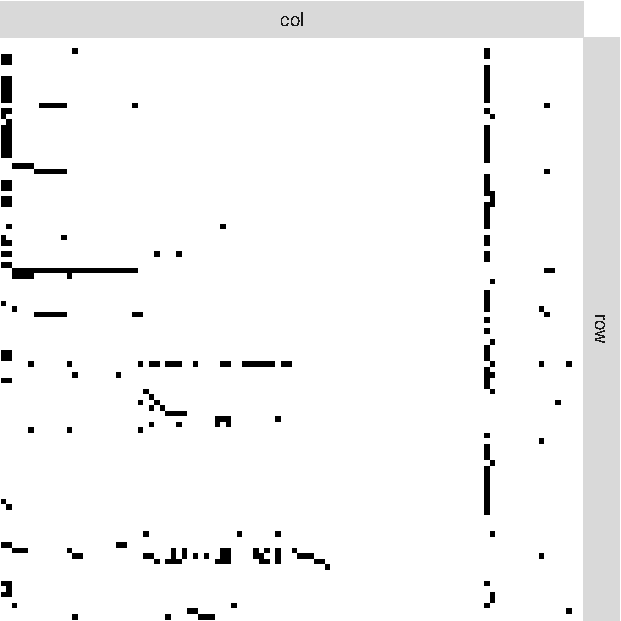
\includegraphics{_main_files/figure-latex/unnamed-chunk-5-1.pdf}

\begin{Shaded}
\begin{Highlighting}[]
\NormalTok{net.mat}\OtherTok{\textless{}{-}}\FunctionTok{graph\_from\_adjacency\_matrix}\NormalTok{(mat,}\AttributeTok{mode=}\StringTok{"directed"}\NormalTok{)}
\end{Highlighting}
\end{Shaded}

TO DO: change the way FWebs is used because it does not compile on Mac and Linux\ldots{}

\section{Networks and associated definitions}\label{networks-and-associated-definitions}

\subsection{What is a network?}\label{what-is-a-network}

Networks (or graphs) are sets of nodes linked by edges.
Edges represent pairwise relationships between nodes.
Edges can be directed or not, weighted or binary (0/1).

\subsection{Networks in ecology}\label{networks-in-ecology}

The main types of networks that you can encounter in ecology:
- the most common: interaction networks (edges are interactions, nodes are species)
- less common: spatial networks (edges are spatial connections, nodes are populations on a map)
- the rarest: assembly networks (edges are transitions between community compositions, nodes are community compositions)

\subsection{Ecological interaction networks}\label{ecological-interaction-networks}

Since biotic interactions are very diverse, many different types of interaction networks can be built (mutualistic, antagonistic, etc.).
The type of data that can be obtained on networks is manifold:
- interaction frequency, especially from field observations (e.g.~how many times a pollinator species is observed on a particular plant species);
- co-abundances or co-occurrences of the species pairs;
- interaction potentials, mostly obtained from experiments (e.g.~arena experiments in which species are put together pairwise to observe interactions)

\subsection{A little history}\label{a-little-history}

The study of ecological interaction networks begun as early as the 50's with some landmark papers like Hutchinson's (Santa Rosalia, etc.) or Paine's series of keystone predation papers. The book of Allee is remarkable as it contains some of the earliest diagrams of food webs.

\subsection{Types of network}\label{types-of-network}

\subsubsection{Unipartite networks}\label{unipartite-networks}

One large class of ecological networks is unipartite networks, i.e.~messy ones in which interactions can occur between any two species. E.g. the Benguela food web of Yodzis (1998).
The function sample\_gnp can generate random unipartite networks using the Erdos-Reyi model, which assumes that any interaction has the same probability to exist.
The plot function of igraph makes basic plots of networks, the layout option helps see things a wee bit more clearly.

\begin{Shaded}
\begin{Highlighting}[]
\NormalTok{net}\OtherTok{\textless{}{-}}\FunctionTok{sample\_gnp}\NormalTok{(}\DecValTok{30}\NormalTok{,}\FloatTok{0.2}\NormalTok{,}\AttributeTok{directed =} \ConstantTok{FALSE}\NormalTok{)}
\FunctionTok{plot}\NormalTok{(net)}
\end{Highlighting}
\end{Shaded}

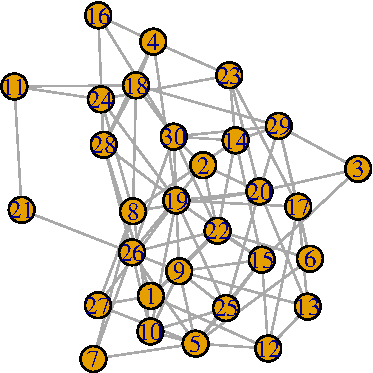
\includegraphics{_main_files/figure-latex/unnamed-chunk-6-1.pdf}

\begin{Shaded}
\begin{Highlighting}[]
\NormalTok{net}\OtherTok{\textless{}{-}}\FunctionTok{sample\_gnp}\NormalTok{(}\DecValTok{30}\NormalTok{,}\FloatTok{0.2}\NormalTok{, }\AttributeTok{directed =}\ConstantTok{TRUE}\NormalTok{)}
\FunctionTok{plot}\NormalTok{(net)}
\end{Highlighting}
\end{Shaded}

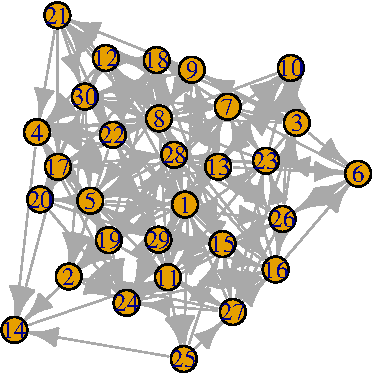
\includegraphics{_main_files/figure-latex/unnamed-chunk-6-2.pdf}

\begin{Shaded}
\begin{Highlighting}[]
\FunctionTok{plot}\NormalTok{(net.mat,}\AttributeTok{layout=}\NormalTok{layout\_with\_mds)}
\end{Highlighting}
\end{Shaded}

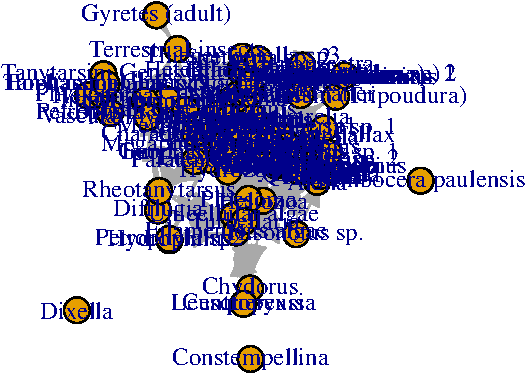
\includegraphics{_main_files/figure-latex/unnamed-chunk-6-3.pdf}

\begin{Shaded}
\begin{Highlighting}[]
\FunctionTok{plot}\NormalTok{(net.mat,}\AttributeTok{layout=}\NormalTok{layout\_as\_tree)}
\end{Highlighting}
\end{Shaded}

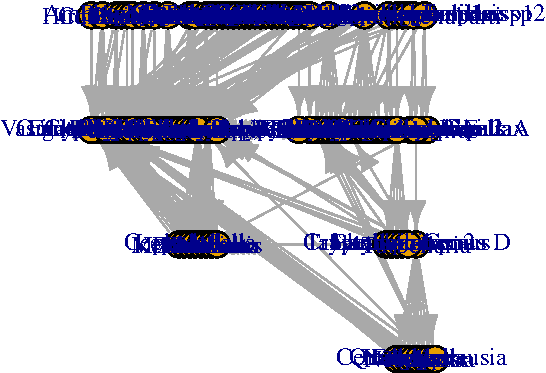
\includegraphics{_main_files/figure-latex/unnamed-chunk-6-4.pdf}

\subsubsection{Multipartite networks}\label{multipartite-networks}

Another large class of networks is the one consisting of multipartite networks, i.e.~networks in which nodes can be partitioned among different levels and nodes only interact among different levels and never within the same level.
Each species/node then has a ``role'' which defines its ``level''.
The most common type of multipartite network encountered in ecology is bipartite network (only two levels) such as plant-pollinator networks.
The function sample\_bipartite generates a random bipartite network using the Erdos-Renyi model.

\begin{Shaded}
\begin{Highlighting}[]
\NormalTok{net}\OtherTok{\textless{}{-}}\FunctionTok{sample\_bipartite}\NormalTok{(}\DecValTok{20}\NormalTok{,}\DecValTok{20}\NormalTok{,}\StringTok{"gnp"}\NormalTok{,}\FloatTok{0.1}\NormalTok{)}
\FunctionTok{plot}\NormalTok{(net,}\AttributeTok{layout=}\NormalTok{layout\_as\_bipartite)}
\end{Highlighting}
\end{Shaded}

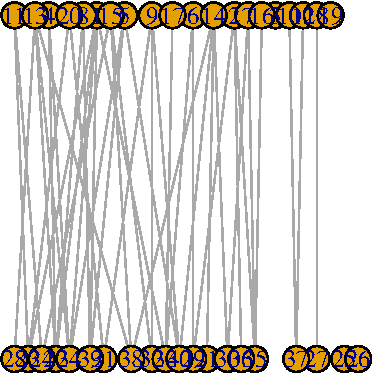
\includegraphics{_main_files/figure-latex/unnamed-chunk-7-1.pdf}

\section{Representation of networks}\label{representation-of-networks}

\subsection{Binary networks}\label{binary-networks}

Having networks as collections of nodes and edges can be insightful, but to make computations on networks, one needs to express them using useful mathematical object. The easiest way is to express a network as a matrix called the adjacency matrix. The element \(a_{ij}\) of an adjacency matrix is equal to 1 iff there exists an interaction between species \(i\) and \(j\). This also works for directed networks.
The function sample\_grg given here generates a random graph based on a random geometric graph process -- it assumes that nodes have coordinates in 2D within a 1 x 1 square and interactions exist when the distance between two nodes is less than a given threshold (here, 0.2).
The function as\_adjacency\_matrix yields the adjacency matrix of the network.

\begin{Shaded}
\begin{Highlighting}[]
\NormalTok{net}\OtherTok{\textless{}{-}}\FunctionTok{sample\_grg}\NormalTok{(}\DecValTok{30}\NormalTok{, }\FloatTok{0.2}\NormalTok{)}
\FunctionTok{as\_adjacency\_matrix}\NormalTok{(net)}
\end{Highlighting}
\end{Shaded}

\begin{verbatim}
## 30 x 30 sparse Matrix of class "dgCMatrix"
##                                                                  
##  [1,] . . 1 . . . . . . . . . . . . . . . . . . . . . . . . . . .
##  [2,] . . . 1 . 1 . . . . . . . . . . . . . . . . . . . . . . . .
##  [3,] 1 . . . 1 . 1 . . . . . . . . . . . . . . . . . . . . . . .
##  [4,] . 1 . . 1 1 . 1 . . 1 . . . . . . . . . . . . . . . . . . .
##  [5,] . . 1 1 . . 1 1 . . 1 . . . . . . . . . . . . . . . . . . .
##  [6,] . 1 . 1 . . . . . . . . . . . . . . . . . . . . . . . . . .
##  [7,] . . 1 . 1 . . 1 . . 1 . 1 1 1 . . . . . . . . . . . . . . .
##  [8,] . . . 1 1 . 1 . . . 1 . . . . 1 . . . . . . . . . . . . . .
##  [9,] . . . . . . . . . . . 1 . . . . . . . . . . . . . . . . . .
## [10,] . . . . . . . . . . . . . . . . . . . . . . . . . . . . . .
## [11,] . . . 1 1 . 1 1 . . . . 1 . 1 1 . . . . . . . . . . . . . .
## [12,] . . . . . . . . 1 . . . . 1 . . 1 . . . . . . . . . . . . .
## [13,] . . . . . . 1 . . . 1 . . 1 1 . 1 . . . . . . . . . . . . .
## [14,] . . . . . . 1 . . . . 1 1 . 1 . 1 . . . . . . . . . . . . .
## [15,] . . . . . . 1 . . . 1 . 1 1 . . 1 . . . . . . . . . . . . .
## [16,] . . . . . . . 1 . . 1 . . . . . . . . . . . . . . . . . . .
## [17,] . . . . . . . . . . . 1 1 1 1 . . . 1 . . . . . . . . . . .
## [18,] . . . . . . . . . . . . . . . . . . 1 . . . . . . . . . . .
## [19,] . . . . . . . . . . . . . . . . 1 1 . . . . . . . . . . . .
## [20,] . . . . . . . . . . . . . . . . . . . . 1 . . 1 1 . . . . .
## [21,] . . . . . . . . . . . . . . . . . . . 1 . . . 1 1 1 . 1 . .
## [22,] . . . . . . . . . . . . . . . . . . . . . . 1 . . . . . . .
## [23,] . . . . . . . . . . . . . . . . . . . . . 1 . . . . . . . .
## [24,] . . . . . . . . . . . . . . . . . . . 1 1 . . . 1 1 1 1 1 .
## [25,] . . . . . . . . . . . . . . . . . . . 1 1 . . 1 . 1 1 1 1 .
## [26,] . . . . . . . . . . . . . . . . . . . . 1 . . 1 1 . 1 1 1 .
## [27,] . . . . . . . . . . . . . . . . . . . . . . . 1 1 1 . 1 . .
## [28,] . . . . . . . . . . . . . . . . . . . . 1 . . 1 1 1 1 . 1 .
## [29,] . . . . . . . . . . . . . . . . . . . . . . . 1 1 1 . 1 . .
## [30,] . . . . . . . . . . . . . . . . . . . . . . . . . . . . . .
\end{verbatim}

\subsection{Weighted networks}\label{weighted-networks}

When a network is weighted, the weighted adjacency matrix represents not only the existing/absent interactions, but also how strong these interactions are.
Here, we create random weights for the edges of network ``net'' using a Poisson distribution of mean 2.
Adding ``{[},{]}'' after the name of network also yields the adjacency matrix.

\begin{Shaded}
\begin{Highlighting}[]
\FunctionTok{E}\NormalTok{(net)}\SpecialCharTok{$}\NormalTok{weight}\OtherTok{\textless{}{-}}\FunctionTok{rpois}\NormalTok{(}\FunctionTok{length}\NormalTok{(}\FunctionTok{E}\NormalTok{(net)),}\DecValTok{2}\NormalTok{)}
\NormalTok{net[,]}
\end{Highlighting}
\end{Shaded}

\begin{verbatim}
## 30 x 30 sparse Matrix of class "dgCMatrix"
##                                                                  
##  [1,] . . 0 . . . . . . . . . . . . . . . . . . . . . . . . . . .
##  [2,] . . . 3 . 3 . . . . . . . . . . . . . . . . . . . . . . . .
##  [3,] 0 . . . 3 . 3 . . . . . . . . . . . . . . . . . . . . . . .
##  [4,] . 3 . . 4 2 . 8 . . 1 . . . . . . . . . . . . . . . . . . .
##  [5,] . . 3 4 . . 1 2 . . 2 . . . . . . . . . . . . . . . . . . .
##  [6,] . 3 . 2 . . . . . . . . . . . . . . . . . . . . . . . . . .
##  [7,] . . 3 . 1 . . 1 . . 0 . 0 5 0 . . . . . . . . . . . . . . .
##  [8,] . . . 8 2 . 1 . . . 1 . . . . 1 . . . . . . . . . . . . . .
##  [9,] . . . . . . . . . . . 2 . . . . . . . . . . . . . . . . . .
## [10,] . . . . . . . . . . . . . . . . . . . . . . . . . . . . . .
## [11,] . . . 1 2 . 0 1 . . . . 2 . 0 3 . . . . . . . . . . . . . .
## [12,] . . . . . . . . 2 . . . . 3 . . 1 . . . . . . . . . . . . .
## [13,] . . . . . . 0 . . . 2 . . 0 3 . 0 . . . . . . . . . . . . .
## [14,] . . . . . . 5 . . . . 3 0 . 3 . 0 . . . . . . . . . . . . .
## [15,] . . . . . . 0 . . . 0 . 3 3 . . 1 . . . . . . . . . . . . .
## [16,] . . . . . . . 1 . . 3 . . . . . . . . . . . . . . . . . . .
## [17,] . . . . . . . . . . . 1 0 0 1 . . . 1 . . . . . . . . . . .
## [18,] . . . . . . . . . . . . . . . . . . 2 . . . . . . . . . . .
## [19,] . . . . . . . . . . . . . . . . 1 2 . . . . . . . . . . . .
## [20,] . . . . . . . . . . . . . . . . . . . . 1 . . 5 1 . . . . .
## [21,] . . . . . . . . . . . . . . . . . . . 1 . . . 3 1 2 . 1 . .
## [22,] . . . . . . . . . . . . . . . . . . . . . . 2 . . . . . . .
## [23,] . . . . . . . . . . . . . . . . . . . . . 2 . . . . . . . .
## [24,] . . . . . . . . . . . . . . . . . . . 5 3 . . . 4 2 2 0 0 .
## [25,] . . . . . . . . . . . . . . . . . . . 1 1 . . 4 . 1 1 4 4 .
## [26,] . . . . . . . . . . . . . . . . . . . . 2 . . 2 1 . 1 3 2 .
## [27,] . . . . . . . . . . . . . . . . . . . . . . . 2 1 1 . 0 . .
## [28,] . . . . . . . . . . . . . . . . . . . . 1 . . 0 4 3 0 . 2 .
## [29,] . . . . . . . . . . . . . . . . . . . . . . . 0 4 2 . 2 . .
## [30,] . . . . . . . . . . . . . . . . . . . . . . . . . . . . . .
\end{verbatim}

\subsection{Network matrices}\label{network-matrices}

Quite naturally, if a network is undirected, its adjacency matrix will be symmetric. When a network is directed, it will not necessarily be so.
One tricky item to keep in mind: sometimes food webs can be represented not using an adjacency matrix, but rather using an ``energy flux'' matrix which represents interactions as an antisymmetric matrix of +1's and -1's.
Adjacency matrices can be binary or real-valued (if they represent interaction weights).
A source of confusion can be the difference between adjacency and incidence matrices.

\subsection{Matrices for multipartite networks}\label{matrices-for-multipartite-networks}

In bipartite networks, the diagonal blocks of the adjacency matrix are full of 0 only. It is thus more useful to only look at the (rectangle) non-zero off-diagonal blocks, which are called the incidence matrix in ecology (or bi-adjacency matrix in other disciplines).
The function as\_biadjacency\_matrix of igraph extracts this matrix from a bipartite network.

\begin{Shaded}
\begin{Highlighting}[]
\NormalTok{net}\OtherTok{\textless{}{-}}\FunctionTok{sample\_bipartite}\NormalTok{(}\DecValTok{4}\NormalTok{,}\DecValTok{4}\NormalTok{,}\StringTok{"gnm"}\NormalTok{,}\AttributeTok{m=}\DecValTok{8}\NormalTok{)}
\NormalTok{net[,]}
\end{Highlighting}
\end{Shaded}

\begin{verbatim}
## 8 x 8 sparse Matrix of class "dgCMatrix"
##                     
## [1,] . . . . 1 1 . .
## [2,] . . . . 1 1 1 .
## [3,] . . . . . . 1 1
## [4,] . . . . 1 . . .
## [5,] 1 1 . 1 . . . .
## [6,] 1 1 . . . . . .
## [7,] . 1 1 . . . . .
## [8,] . . 1 . . . . .
\end{verbatim}

\begin{Shaded}
\begin{Highlighting}[]
\FunctionTok{as\_biadjacency\_matrix}\NormalTok{(net)}
\end{Highlighting}
\end{Shaded}

\begin{verbatim}
##   5 6 7 8
## 1 1 1 0 0
## 2 1 1 1 0
## 3 0 0 1 1
## 4 1 0 0 0
\end{verbatim}

\subsection{Degrees}\label{degrees}

A basic element of representation of networks is the degree of a node.
The degree of a node is the number of interactions it shares with other nodes.
For undirected networks, this definition is straightforward and corresponds to row- or column-sums of the binary adjacency matrix.
For directed networks, one actually needs to define the in-degree and out-degree of each node, which correspond respectively to the number of incoming and outgoing edges.
The function degree of igraph computes all of these using the argument called mode.

\begin{Shaded}
\begin{Highlighting}[]
\FunctionTok{degree}\NormalTok{(net)}
\end{Highlighting}
\end{Shaded}

\begin{verbatim}
## [1] 2 3 2 1 3 2 2 1
\end{verbatim}

\begin{Shaded}
\begin{Highlighting}[]
\FunctionTok{degree}\NormalTok{(net,}\AttributeTok{mode=}\StringTok{"in"}\NormalTok{)}
\end{Highlighting}
\end{Shaded}

\begin{verbatim}
## [1] 2 3 2 1 3 2 2 1
\end{verbatim}

\begin{Shaded}
\begin{Highlighting}[]
\FunctionTok{degree}\NormalTok{(net,}\AttributeTok{mode=}\StringTok{"out"}\NormalTok{)}
\end{Highlighting}
\end{Shaded}

\begin{verbatim}
## [1] 2 3 2 1 3 2 2 1
\end{verbatim}

The degree distribution corresponds to the realized empirical distribution of degrees in the network. It can be obtained using a variety of functions, including degree\_distribution in igraph.

\begin{Shaded}
\begin{Highlighting}[]
\FunctionTok{hist}\NormalTok{(}\FunctionTok{degree}\NormalTok{(net.mat),}\AttributeTok{breaks=}\DecValTok{0}\SpecialCharTok{:}\FunctionTok{max}\NormalTok{(}\FunctionTok{degree}\NormalTok{(net.mat)))}
\end{Highlighting}
\end{Shaded}

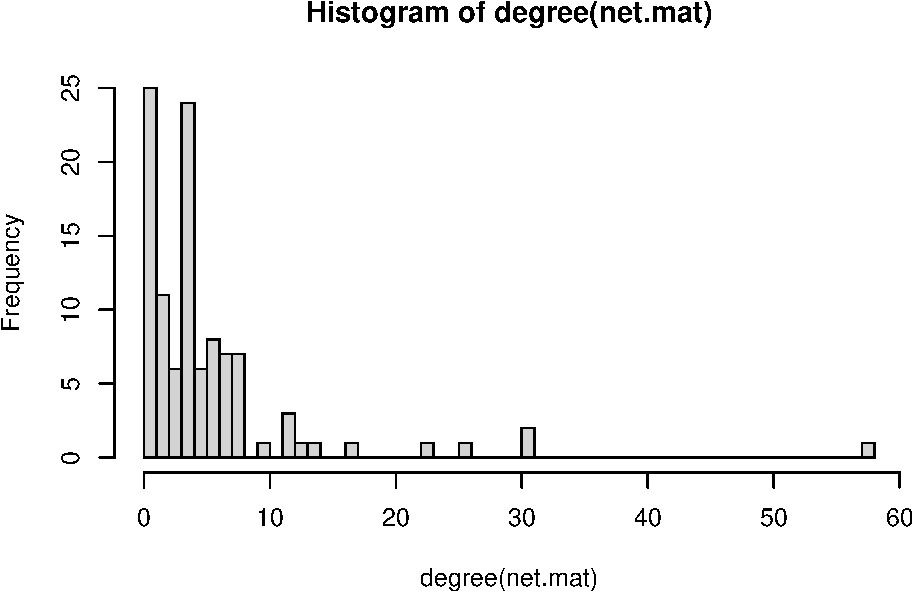
\includegraphics{_main_files/figure-latex/unnamed-chunk-12-1.pdf}

\begin{Shaded}
\begin{Highlighting}[]
\FunctionTok{plot}\NormalTok{(}\FunctionTok{degree\_distribution}\NormalTok{(net.mat, }\AttributeTok{cumulative =} \ConstantTok{TRUE}\NormalTok{))}
\end{Highlighting}
\end{Shaded}

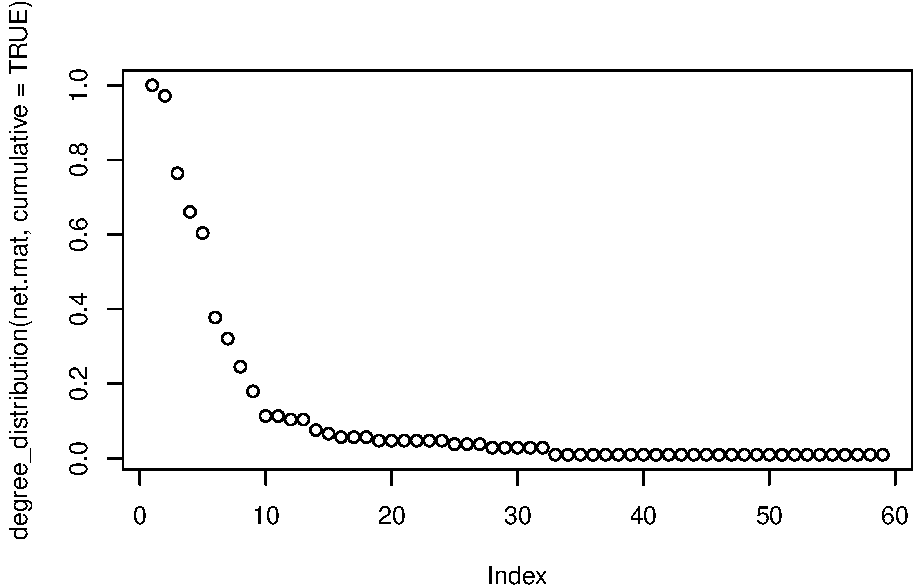
\includegraphics{_main_files/figure-latex/unnamed-chunk-12-2.pdf}

\subsection{Connectance}\label{connectance}

Connectance is an important notion. It is defined as the proportion of possible interactions that really exist. There are plenty of ways to implement its computation (e.g.~using mean), but it is important to correct these according to the impossible interactions (e.g.~correcting for self-links or edges within levels in bipartite networks).

\begin{Shaded}
\begin{Highlighting}[]
\NormalTok{conn}\OtherTok{\textless{}{-}}\FunctionTok{mean}\NormalTok{(}\FunctionTok{as.matrix}\NormalTok{(net.mat[,]))}
\NormalTok{conn}
\end{Highlighting}
\end{Shaded}

\begin{verbatim}
## [1] 0.02669989
\end{verbatim}

\section{Crash course: matrices, eigenvalues, Jacobian matrix}\label{crash-course-matrices-eigenvalues-jacobian-matrix}

\subsection{Crash course: matrices}\label{crash-course-matrices}

Matrices are mathematical objects that represent tables, i.e.~have rows and columns. The element at row \(i\) and column \(j\) of matrix \(M\) is often noted \(m_{ij}\).
Matrices and vectors follow a strange multiplication operation, noted with \%\emph{\% in R (rather than } which encodes a more plastic multiplication operation).

\begin{Shaded}
\begin{Highlighting}[]
\NormalTok{m}\OtherTok{\textless{}{-}}\FunctionTok{matrix}\NormalTok{(}\FunctionTok{rbinom}\NormalTok{(}\DecValTok{9}\NormalTok{,}\DecValTok{1}\NormalTok{,}\FloatTok{0.5}\NormalTok{),}\AttributeTok{nrow=}\DecValTok{3}\NormalTok{)}
\NormalTok{x}\OtherTok{\textless{}{-}}\FunctionTok{rnorm}\NormalTok{(}\DecValTok{3}\NormalTok{)}
\NormalTok{m}\SpecialCharTok{*}\NormalTok{x}
\end{Highlighting}
\end{Shaded}

\begin{verbatim}
##            [,1]       [,2]      [,3]
## [1,] 0.09299545 0.09299545 0.0000000
## [2,] 0.24709379 0.00000000 0.2470938
## [3,] 0.01487206 0.00000000 0.0000000
\end{verbatim}

\begin{Shaded}
\begin{Highlighting}[]
\NormalTok{m}\SpecialCharTok{\%*\%}\NormalTok{x}
\end{Highlighting}
\end{Shaded}

\begin{verbatim}
##            [,1]
## [1,] 0.34008924
## [2,] 0.10786751
## [3,] 0.09299545
\end{verbatim}

\subsection{Crash course: matrix eigenvalues}\label{crash-course-matrix-eigenvalues}

All matrices are associated with a set of values called ``eigenvalues'' which represent the ``multiplicators'' of the matrix. Each of these eigenvalues \(\lambda\) is associated to eigenvectors \(x\) such that multiplying \(x\) by the matrix \(M\) results in only multiplying \(x\) by \(\lambda\):
\[M.x = \lambda x\]

The collection of eigenvalues of \(M\) is called its spectrum. The spectrum is always finite and has at most a number of distinct elements equal to the smallest dimension of \(M\).

The function eigen yields the eigensystem (eigenvalues and eigenvectors) of a matrix.

\begin{Shaded}
\begin{Highlighting}[]
\FunctionTok{eigen}\NormalTok{(m)}
\end{Highlighting}
\end{Shaded}

\begin{verbatim}
## eigen() decomposition
## $values
## [1]  1.8392868+0.0000000i -0.4196434+0.6062907i -0.4196434-0.6062907i
## 
## $vectors
##               [,1]                  [,2]                  [,3]
## [1,] -0.7071068+0i  0.4024298+0.1718667i  0.4024298-0.1718667i
## [2,] -0.5934654+0i -0.6755079+0.0000000i -0.6755079+0.0000000i
## [3,] -0.3844462+0i -0.1189573-0.5814209i -0.1189573+0.5814209i
\end{verbatim}

\subsection{Crash course: Jacobian matrices}\label{crash-course-jacobian-matrices}

A set of ordinary differential equations (ODEs), such as those given by Lotka-Volterra equations, can be written in compact form as:

\[\frac{d\overrightarrow{x}}{dt} = \overrightarrow{F}\left(\overrightarrow{x} \right)\]

Let us assume that there exists an equilibrium \(\overrightarrow{x}^*\) for this system. If we want to assess whether this equilibrium is stable, we need to linearize the dynamics around the equilibrium:

\[\frac{d\left( \overrightarrow{x}-\overrightarrow{x}^*\right)}{dt} \approx J\left(\overrightarrow{x}^*\right).\left( \overrightarrow{x}-\overrightarrow{x}^*\right)\]

The matrix \(J\left(\overrightarrow{x}^*\right)\) is called the Jacobian matrix of the dynamical system at the equilibirum \(\overrightarrow{x}^*\)
The expression for eh Jacobian matrix is obtained using the partial derivatives of the different components of \(\overrightarrow{F}\):
\[J\left(\overrightarrow{x}^*\right) = \left.\left(\partial F_i/\partial x_j\right)\right\rvert_{x=x^*}\]

Formal computations of Jacobian matrices can be done with R using the package calculus:

\begin{Shaded}
\begin{Highlighting}[]
\CommentTok{\#jacobian(c("r*n1*(1{-}n1/k){-}a*n1*n2/(1+h*n1)","b*n1*n2/(1+h*n1){-}d*n2"), var = c("n1", "n2"))}
\end{Highlighting}
\end{Shaded}

\section{Theories and notable results}\label{theories-and-notable-results}

\subsection{Lotka-Volterra and networks}\label{lotka-volterra-and-networks}

This is the classic Lotka-Volterra system, given for a dimensionless system (i.e.~the coefficient of self-feedback are all set to 1):
\[\frac{dx_i}{dt} = x_i \left[ r_i - x_i + \sum_j a_{ij}x_j\right]\]
This system of ODEs can be seen as describing the dynamics of a network of species, with matrix \(A\) as its ``weighted'' adjacency matrix.

\subsection{May's stability result}\label{mays-stability-result}

In the 70's, Sir Robert May published a very important mathematical ecology result which shook some of the beliefs ecologists had at that time.
The idea is to assume that a community consists of \(S\) species and that species abundances of these species are fixed at an equilibrium value \(\overrightarrow{x}^*\). May's approach asks the question: what should happen if elements of the Jacobian matrix were randomly drawn according to a simple distribution? More precisely, May assumed that diagonal elements of the Jacobian were equal (or similar) and negative, while the off-diagonal elements had a probability \(c\) (the connectance) of being non-zero, and if not equal to zero, followed a normal distribution of mean 0 and standard deviation \(\sigma\).
The result of May thus stipulates that the equilibrium can only be stable when
\[\begin{equation} 
\sigma \sqrt{cS} < -\overline{J_{ii}} 
\end{equation}\]

This result can be explained geometrically (based on the circular law): for a random matrix with this particular distribution of off-diagonal elements, the distribution of eigenvalues will be enclosed in a disk of center \(\left(-\overline{J_{ii}},0\right)\) and radius \(\sigma \sqrt{cS}\) in the complex plane. For all eigenvalues to have negative real parts, the radius of this disk should be less than the distance between (0,0) and its center.

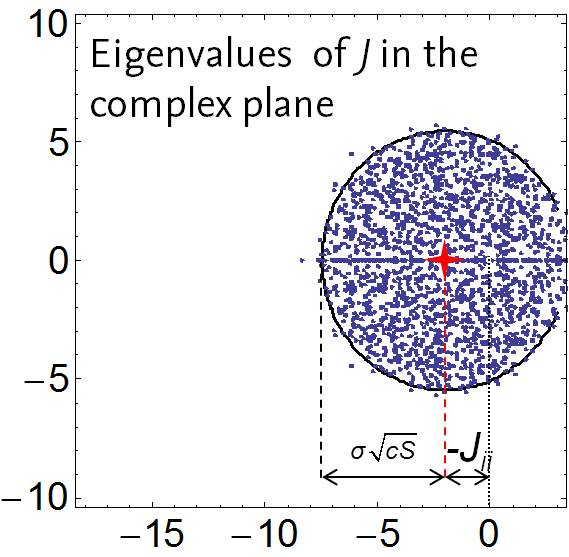
\includegraphics[width=7.9in]{fig06Networks/May}

\begin{Shaded}
\begin{Highlighting}[]
\NormalTok{m}\OtherTok{\textless{}{-}}\FunctionTok{matrix}\NormalTok{(}\FunctionTok{rnorm}\NormalTok{(}\DecValTok{10}\SpecialCharTok{\^{}}\DecValTok{6}\NormalTok{),}\AttributeTok{nrow=}\DecValTok{10}\SpecialCharTok{\^{}}\DecValTok{3}\NormalTok{)}
\FunctionTok{plot}\NormalTok{(}\FunctionTok{eigen}\NormalTok{(m)}\SpecialCharTok{$}\NormalTok{values,}\AttributeTok{asp=}\DecValTok{1}\NormalTok{)}
\end{Highlighting}
\end{Shaded}

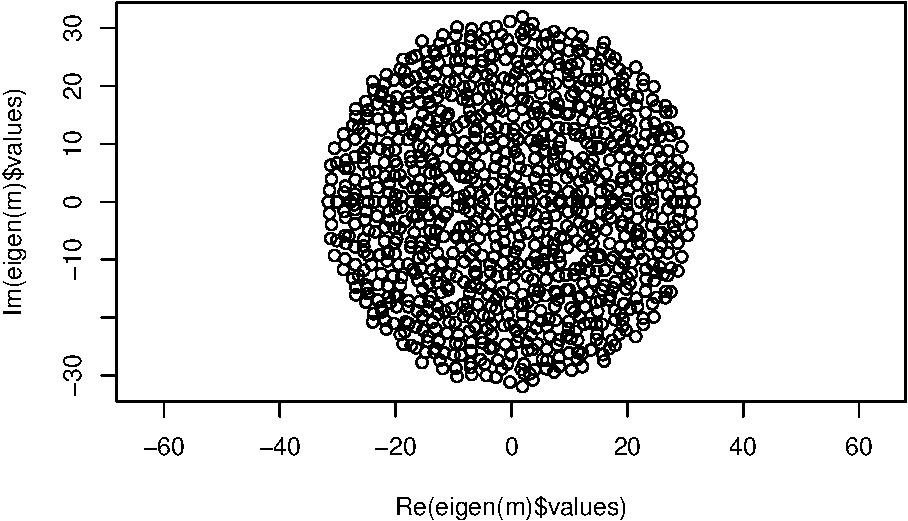
\includegraphics{_main_files/figure-latex/unnamed-chunk-18-1.pdf}
This result can be interpreted as follows: for a given equilibrium to be stable, it should have low diversity and/or low connectance and/or a low variability of non-diagonal Jacobian elements (i.e.~feedbacks among species abundances) and/or highly negative diagonal Jacobian elements (i.e.~strong negative feedbacks of species upon themselves).

Intuitively, this does not seem to conform to reality: we see species-rich systems in which species interact relatively strongly and not too sparsely, without intense self-regulation\ldots{}
So, some of the assumptions must be false and we can look for changes to these assumptions:
- dynamics could be transient rather than at equilibrium
- interactions might be structured and not completely random (see Claire's talk)

\subsection{Feasibility vs.~stability}\label{feasibility-vs.-stability}

One other strong argument contradicting May's result is the following: in many cases, it might actually be more difficult to obtain an equilibrium including all species (i.e.~have feasibility) than for this equilibrium to be stable.
For instance, Bizeul \& Najim proved that in a certain class of LV systems, feasibility is obtained only when
\[\sigma \sqrt{2Slog(S)} < -\overline{J_{ii}}\]
where \(\sigma\) is the standard deviation of the LV matrix (not the Jacobian matrix) and the connectance is merged into \(\sigma^2\).

In the simulation paper of L. Stone, similar results were obtained -- here stability (on the left) is lost after feasibility (on the right) when increasing of a parameter (\(\gamma\)) which is proportional to our \(\sigma\).

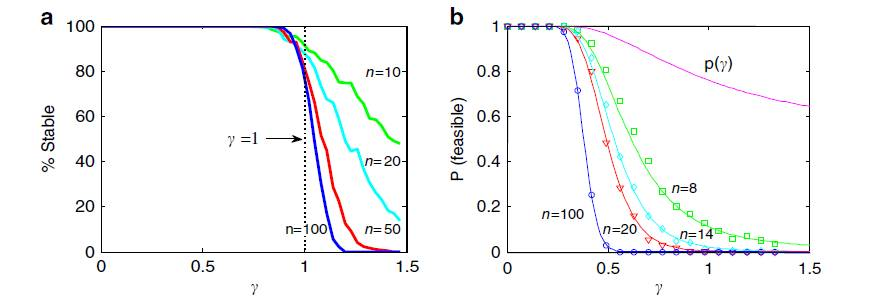
\includegraphics[width=12.11in]{fig06Networks/Stone}

\subsection{Food web invariants}\label{food-web-invariants}

In the 80-90's, one important goal of interaction network research was to find invariant properties, i.e.~statistics or metrics that did not vary among food webs. With this goal in mind, two models were proposed.
First, the cascade model of Cohen \& Briand proposed that predators only eat a rather fixed number of prey species. This corresponds to predators eating prey that are are smaller than them with probability \(c/S\) (\(c\) being a fixed parameter), so that connectance decreases as \(1/S\).

\begin{Shaded}
\begin{Highlighting}[]
\NormalTok{m}\OtherTok{\textless{}{-}}\FunctionTok{cascade\_matrix}\NormalTok{(}\DecValTok{10}\NormalTok{,}\DecValTok{20}\NormalTok{)}
\FunctionTok{sum}\NormalTok{(m)}\SpecialCharTok{/}\NormalTok{(}\FunctionTok{dim}\NormalTok{(m)[}\DecValTok{1}\NormalTok{]}\SpecialCharTok{*}\NormalTok{(}\FunctionTok{dim}\NormalTok{(m)[}\DecValTok{1}\NormalTok{]}\SpecialCharTok{{-}}\DecValTok{1}\NormalTok{))}
\end{Highlighting}
\end{Shaded}

\begin{verbatim}
## [1] 0.2710526
\end{verbatim}

\begin{Shaded}
\begin{Highlighting}[]
\NormalTok{m}\OtherTok{\textless{}{-}}\FunctionTok{cascade\_matrix}\NormalTok{(}\DecValTok{10}\NormalTok{,}\DecValTok{200}\NormalTok{)}
\FunctionTok{sum}\NormalTok{(m)}\SpecialCharTok{/}\NormalTok{(}\FunctionTok{dim}\NormalTok{(m)[}\DecValTok{1}\NormalTok{]}\SpecialCharTok{*}\NormalTok{(}\FunctionTok{dim}\NormalTok{(m)[}\DecValTok{1}\NormalTok{]}\SpecialCharTok{{-}}\DecValTok{1}\NormalTok{))}
\end{Highlighting}
\end{Shaded}

\begin{verbatim}
## [1] 0.02389447
\end{verbatim}

The second model that was developed to find invariants is the niche model of Williams and Martinez. In this model, all species are supposed to be defined by their size and to eat all species with size contained within an interval centred around a size lower than the predator's.
With the right parameter values, one can use this model to generate a food web that has a given connectance, whatever the number of species in the food web.

\begin{Shaded}
\begin{Highlighting}[]
\NormalTok{niche}\OtherTok{\textless{}{-}}\FunctionTok{niche\_matrix}\NormalTok{(}\FloatTok{0.2}\NormalTok{,}\DecValTok{100}\NormalTok{)}
\NormalTok{m}\OtherTok{\textless{}{-}}\NormalTok{niche}\SpecialCharTok{$}\NormalTok{matrix}
\FunctionTok{sum}\NormalTok{(m)}\SpecialCharTok{/}\NormalTok{(}\FunctionTok{dim}\NormalTok{(m)[}\DecValTok{1}\NormalTok{]}\SpecialCharTok{\^{}}\DecValTok{2}\NormalTok{)}
\end{Highlighting}
\end{Shaded}

\begin{verbatim}
## [1] 0.1799
\end{verbatim}

\begin{Shaded}
\begin{Highlighting}[]
\NormalTok{niche}\OtherTok{\textless{}{-}}\FunctionTok{niche\_matrix}\NormalTok{(}\FloatTok{0.2}\NormalTok{,}\DecValTok{200}\NormalTok{)}
\NormalTok{m}\OtherTok{\textless{}{-}}\NormalTok{niche}\SpecialCharTok{$}\NormalTok{matrix}
\FunctionTok{sum}\NormalTok{(m)}\SpecialCharTok{/}\NormalTok{(}\FunctionTok{dim}\NormalTok{(m)[}\DecValTok{1}\NormalTok{]}\SpecialCharTok{\^{}}\DecValTok{2}\NormalTok{)}
\end{Highlighting}
\end{Shaded}

\begin{verbatim}
## [1] 0.198325
\end{verbatim}

\subsection{Generating the niche model}\label{generating-the-niche-model}

Exercise: generate 100 virtual food webs similar to the one described by mat

\begin{Shaded}
\begin{Highlighting}[]
\NormalTok{niches}\OtherTok{\textless{}{-}}\FunctionTok{lapply}\NormalTok{(}\DecValTok{1}\SpecialCharTok{:}\DecValTok{100}\NormalTok{,}\ControlFlowTok{function}\NormalTok{(x) }\FunctionTok{niche\_matrix}\NormalTok{(conn,}\FunctionTok{dim}\NormalTok{(mat)[}\DecValTok{1}\NormalTok{]))}
\NormalTok{ms}\OtherTok{\textless{}{-}}\FunctionTok{lapply}\NormalTok{(}\DecValTok{1}\SpecialCharTok{:}\DecValTok{100}\NormalTok{,}\ControlFlowTok{function}\NormalTok{(x) niches[[x]]}\SpecialCharTok{$}\NormalTok{matrix)}
\end{Highlighting}
\end{Shaded}

\subsection{Robustness to secondary extinctions}\label{robustness-to-secondary-extinctions}

The general idea is to assume that when a species is removed from a network, the species interacting with it could go extinct (secondary extinction).
Robustness analysis then consists in assessing how many species are lost when R species are removed.
The most used indicator of robustness is the R50 which is the percentage of species on needs to remove from a web to lose 50\% of its species.

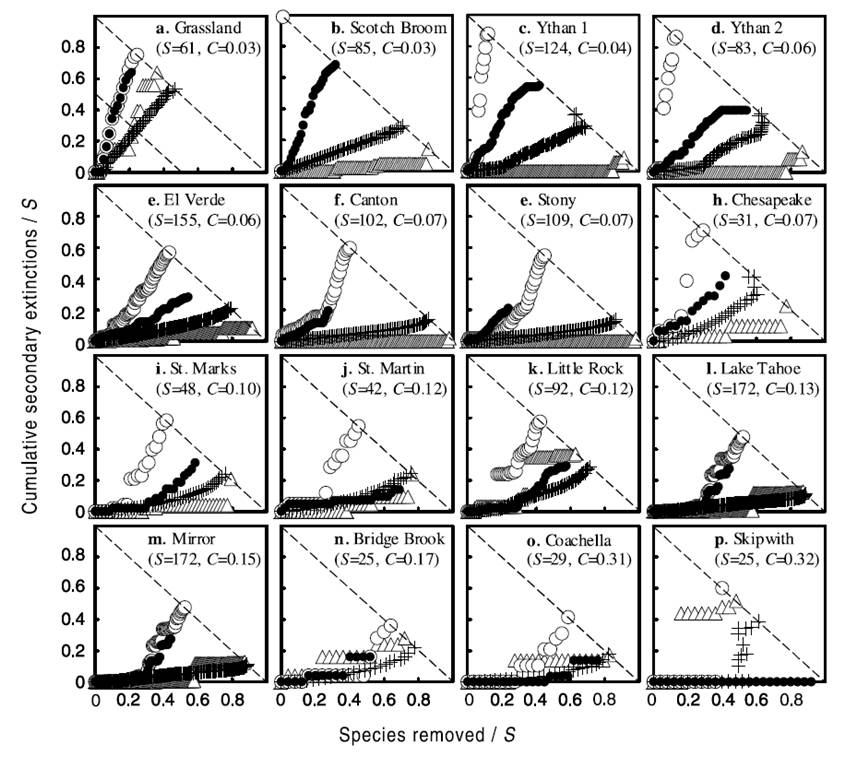
\includegraphics[width=11.92in]{fig06Networks/Dunne1}

In the paper of J. Dunne and collaborators, they used examples based on a variety of datasets. The basic rule then is that a species go extinct when it loses all its prey items (except itself if it is cannibalistic).
One can obtain different scenarios based on how removed species are chosen (intentionality: how strongly the species' degree changes its probability of being drawn randomly as the next one to be removed).

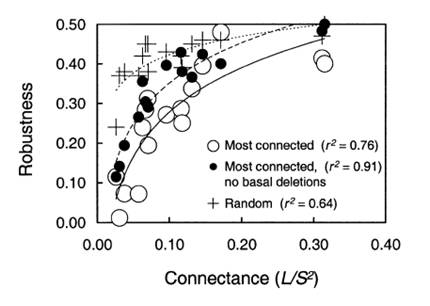
\includegraphics[width=5.97in]{fig06Networks/Dunne2}

\begin{Shaded}
\begin{Highlighting}[]
\NormalTok{net}\OtherTok{\textless{}{-}}\FunctionTok{graph\_from\_adjacency\_matrix}\NormalTok{(m,}\AttributeTok{mode=}\StringTok{"directed"}\NormalTok{)}
\NormalTok{i\_index }\OtherTok{\textless{}{-}} \FunctionTok{seq}\NormalTok{(}\AttributeTok{from =} \DecValTok{0}\NormalTok{, }\AttributeTok{to =} \DecValTok{1}\NormalTok{, }\AttributeTok{by =}\FloatTok{0.1}\NormalTok{)}
\NormalTok{i\_index }\OtherTok{\textless{}{-}} \FunctionTok{head}\NormalTok{(i\_index,}\SpecialCharTok{{-}}\DecValTok{1}\NormalTok{)}
\NormalTok{prob\_exp}\OtherTok{\textless{}{-}}\FunctionTok{exponent.removal}\NormalTok{(net, i\_index)}
\FunctionTok{V}\NormalTok{(net)}\SpecialCharTok{$}\NormalTok{name}\OtherTok{\textless{}{-}}\DecValTok{1}\SpecialCharTok{:}\DecValTok{200}
\FunctionTok{iterate}\NormalTok{(}\AttributeTok{fw\_to\_attack=}\NormalTok{net, prob\_exp, }\AttributeTok{alpha1=}\DecValTok{50}\NormalTok{, }\AttributeTok{iter=}\DecValTok{10}\NormalTok{, i\_index, }\AttributeTok{plot =} \ConstantTok{TRUE}\NormalTok{)}
\end{Highlighting}
\end{Shaded}

\begin{verbatim}
## Iteration 1
\end{verbatim}

\begin{verbatim}
## Iteration 2
\end{verbatim}

\begin{verbatim}
## Iteration 3
\end{verbatim}

\begin{verbatim}
## Iteration 4
\end{verbatim}

\begin{verbatim}
## Iteration 5
\end{verbatim}

\begin{verbatim}
## Iteration 6
\end{verbatim}

\begin{verbatim}
## Iteration 7
\end{verbatim}

\begin{verbatim}
## Iteration 8
\end{verbatim}

\begin{verbatim}
## Iteration 9
\end{verbatim}

\begin{verbatim}
## Iteration 10
\end{verbatim}

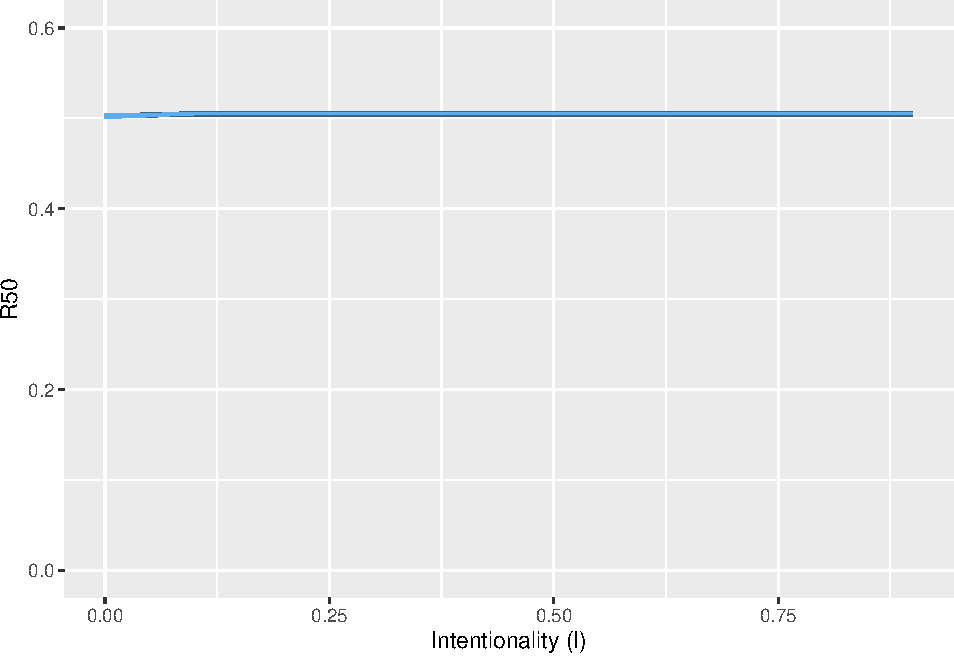
\includegraphics{_main_files/figure-latex/unnamed-chunk-25-1.pdf}

\begin{verbatim}
##    i_index  meanR         sdR lower.bound upper.bound
## 1      0.0 0.5025 0.002635231   0.5008667   0.5041333
## 2      0.1 0.5050 0.000000000   0.5050000   0.5050000
## 3      0.2 0.5050 0.000000000   0.5050000   0.5050000
## 4      0.3 0.5050 0.000000000   0.5050000   0.5050000
## 5      0.4 0.5050 0.000000000   0.5050000   0.5050000
## 6      0.5 0.5050 0.000000000   0.5050000   0.5050000
## 7      0.6 0.5050 0.000000000   0.5050000   0.5050000
## 8      0.7 0.5050 0.000000000   0.5050000   0.5050000
## 9      0.8 0.5050 0.000000000   0.5050000   0.5050000
## 10     0.9 0.5050 0.000000000   0.5050000   0.5050000
\end{verbatim}

\section{A quick primer on network statistics}\label{a-quick-primer-on-network-statistics}

\subsection{Degree distributions}\label{degree-distributions}

Basically, one can do three things with degree distributions:
- compute them empirically
- generate networks similar to one that is observed using its degree sequence
- compare the degree distribution to benchmark distributions of integers (Poisson, power law, \ldots) or of degrees of well-known random networks (Erdos-Renyi, random geometric graph, Watts-Strogatz\ldots)

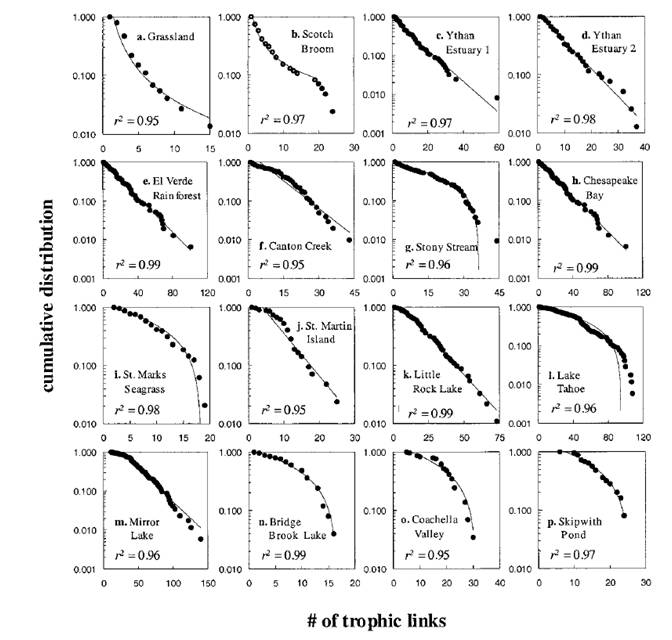
\includegraphics[width=9.33in]{fig06Networks/Dunne3}

\begin{Shaded}
\begin{Highlighting}[]
\NormalTok{net}\OtherTok{\textless{}{-}}\FunctionTok{graph\_from\_adjacency\_matrix}\NormalTok{(m)}
\FunctionTok{hist}\NormalTok{(}\FunctionTok{degree}\NormalTok{(net),}\AttributeTok{breaks=}\DecValTok{0}\SpecialCharTok{:}\FunctionTok{max}\NormalTok{(}\FunctionTok{degree}\NormalTok{(net)))}
\end{Highlighting}
\end{Shaded}

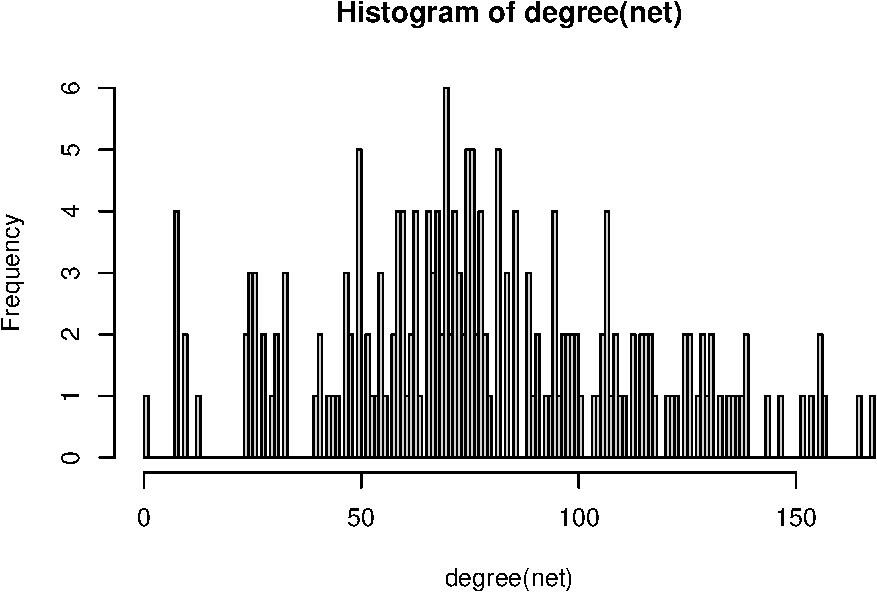
\includegraphics{_main_files/figure-latex/unnamed-chunk-27-1.pdf}

\begin{Shaded}
\begin{Highlighting}[]
\FunctionTok{plot}\NormalTok{(}\FunctionTok{degree\_distribution}\NormalTok{(net, }\AttributeTok{cumulative =} \ConstantTok{TRUE}\NormalTok{))}
\end{Highlighting}
\end{Shaded}

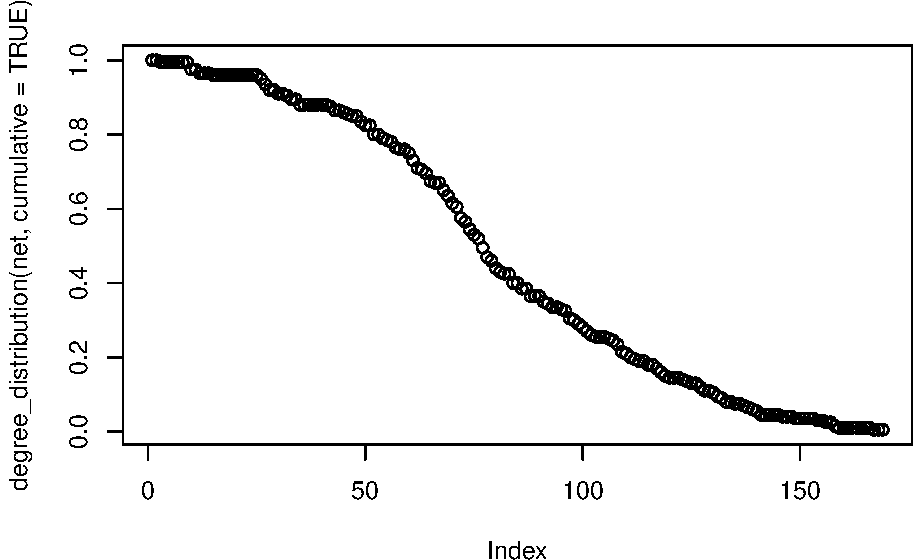
\includegraphics{_main_files/figure-latex/unnamed-chunk-27-2.pdf}

\begin{Shaded}
\begin{Highlighting}[]
\NormalTok{net}\OtherTok{\textless{}{-}}\FunctionTok{sample\_degseq}\NormalTok{(}\FunctionTok{degree}\NormalTok{(net),}\AttributeTok{method =} \StringTok{"vl"}\NormalTok{)}

\FunctionTok{mean}\NormalTok{(}\FunctionTok{degree}\NormalTok{(net))}
\end{Highlighting}
\end{Shaded}

\begin{verbatim}
## [1] 79.33
\end{verbatim}

\begin{Shaded}
\begin{Highlighting}[]
\FunctionTok{ks.test}\NormalTok{(}\FunctionTok{degree}\NormalTok{(net),}\StringTok{"pbinom"}\NormalTok{,}\FunctionTok{length}\NormalTok{(}\FunctionTok{V}\NormalTok{(net)),}\FunctionTok{mean}\NormalTok{(}\FunctionTok{degree}\NormalTok{(net))}\SpecialCharTok{/}\FunctionTok{length}\NormalTok{(}\FunctionTok{V}\NormalTok{(net)))}
\end{Highlighting}
\end{Shaded}

\begin{verbatim}
## Warning in ks.test.default(degree(net), "pbinom", length(V(net)),
## mean(degree(net))/length(V(net))): ties should not be present for the
## Kolmogorov-Smirnov test
\end{verbatim}

\begin{verbatim}
## 
##  Asymptotic one-sample Kolmogorov-Smirnov test
## 
## data:  degree(net)
## D = 0.32724, p-value < 2.2e-16
## alternative hypothesis: two-sided
\end{verbatim}

Power laws are among the most popular distributions of degrees discussed in the literature. However, a question worth asking is whether power laws are useful in ecology, i.e.~whether it is actually possible to ascertain power-lawed degrees in ecological networks.
As Stumpf \& Porter (2012) clearly articulated, this would require to have degrees ranging at the very least between 1 and 100 (2 orders of magnitude), which is quite unheard of.

\subsection{Null models / randomizations}\label{null-models-randomizations}

Statistics on networks are hard to test because everything depends on everything else in a network\ldots{}

So to test for extraordinary patterns in a network (or between them), one can resort to two strategies:
- either to define a probabilistic model to build a null hypothesis (e.g.~using the expected degree distribution)
- or to define a null model based on some randomization scheme

One of the most useful and simplest such scheme is the configuration model. Under this null model, edges are randomly reattached to other nodes such that all nodes keep their degrees. This behaves effectively as if all nodes were attached to half-edges which were randomly paired until the resulting network yields no self-link and no double link.

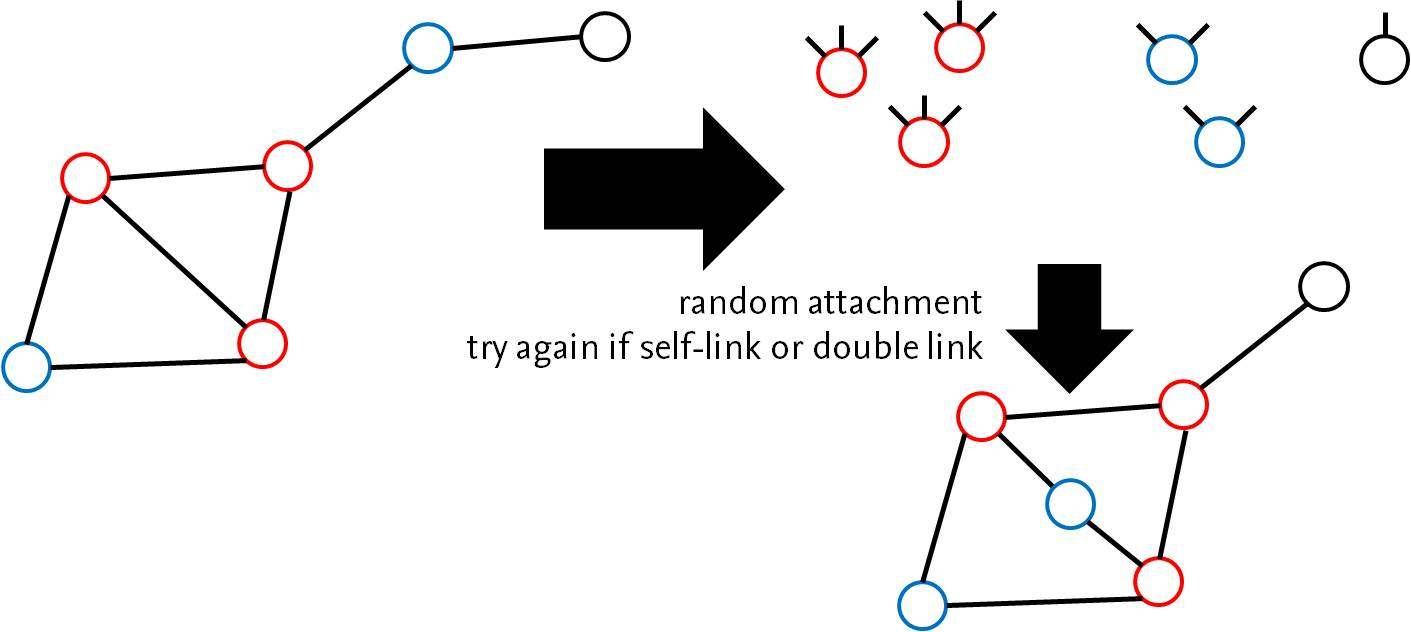
\includegraphics[width=19.6in]{fig06Networks/configuration}

For bipartite binary networks, there is an algorithm (curveball) which yields the configuration model quickly and efficiently.

\begin{Shaded}
\begin{Highlighting}[]
\NormalTok{net}\OtherTok{\textless{}{-}}\FunctionTok{sample\_bipartite}\NormalTok{(}\DecValTok{50}\NormalTok{,}\DecValTok{50}\NormalTok{,}\StringTok{"gnp"}\NormalTok{,}\FloatTok{0.1}\NormalTok{)}
\NormalTok{sample.bip.config}\OtherTok{\textless{}{-}}\FunctionTok{simulate}\NormalTok{(}\FunctionTok{nullmodel}\NormalTok{(}\FunctionTok{as\_incidence\_matrix}\NormalTok{(net),}\StringTok{"curveball"}\NormalTok{),}\AttributeTok{nsim=}\DecValTok{1000}\NormalTok{)}
\end{Highlighting}
\end{Shaded}

\begin{verbatim}
## Warning: `as_incidence_matrix()` was deprecated in igraph 1.6.0.
## i Please use `as_biadjacency_matrix()` instead.
## This warning is displayed once every 8 hours.
## Call `lifecycle::last_lifecycle_warnings()` to see where this warning was
## generated.
\end{verbatim}

\begin{Shaded}
\begin{Highlighting}[]
\FunctionTok{dim}\NormalTok{(sample.bip.config)}
\end{Highlighting}
\end{Shaded}

\begin{verbatim}
## [1]   50   50 1000
\end{verbatim}

For unipartite binary networks, the task is slightly harder, but doable using sample\_degseq.

\begin{Shaded}
\begin{Highlighting}[]
\NormalTok{n}\OtherTok{\textless{}{-}}\DecValTok{200} \CommentTok{\#1000}
\NormalTok{net}\OtherTok{\textless{}{-}}\FunctionTok{sample\_gnp}\NormalTok{(n,}\FloatTok{0.2}\NormalTok{, }\AttributeTok{directed =} \ConstantTok{FALSE}\NormalTok{)}
\NormalTok{sample.config.undirected}\OtherTok{\textless{}{-}}\FunctionTok{lapply}\NormalTok{(}\DecValTok{1}\SpecialCharTok{:}\DecValTok{100}\NormalTok{,}\ControlFlowTok{function}\NormalTok{(x) }\FunctionTok{sample\_degseq}\NormalTok{(}\FunctionTok{degree}\NormalTok{(net), }\AttributeTok{method =} \StringTok{"vl"}\NormalTok{))}
\FunctionTok{length}\NormalTok{(sample.config.undirected)}
\end{Highlighting}
\end{Shaded}

\begin{verbatim}
## [1] 100
\end{verbatim}

For directed networks, it is even worse because we have no indication that the random matrices are all explored and represented fairly among the realizations of the algorithm.

\begin{Shaded}
\begin{Highlighting}[]
\NormalTok{net}\OtherTok{\textless{}{-}}\FunctionTok{sample\_gnp}\NormalTok{(n,}\FloatTok{0.2}\NormalTok{, }\AttributeTok{directed =} \ConstantTok{TRUE}\NormalTok{)}
\NormalTok{sample.config.directed}\OtherTok{\textless{}{-}}\FunctionTok{lapply}\NormalTok{(}\DecValTok{1}\SpecialCharTok{:}\DecValTok{100}\NormalTok{,}\ControlFlowTok{function}\NormalTok{(x) }\FunctionTok{sample\_degseq}\NormalTok{(}\FunctionTok{degree}\NormalTok{(net,}\AttributeTok{mode=}\StringTok{"out"}\NormalTok{), }\FunctionTok{degree}\NormalTok{(net,}\AttributeTok{mode=}\StringTok{"in"}\NormalTok{), }\AttributeTok{method =} \StringTok{"simple.no.multiple"}\NormalTok{))}
\FunctionTok{length}\NormalTok{(sample.config.directed)}
\end{Highlighting}
\end{Shaded}

\begin{verbatim}
## [1] 100
\end{verbatim}

Finally, for any weighted network (bipartite or unipartite), the task is even more difficult.

\subsection{Network structure}\label{network-structure}

Ecological interaction networks can have non-random structures. In ecology, we tend to focus on two such structures: modularity (on the left) and nestedness (on the right).

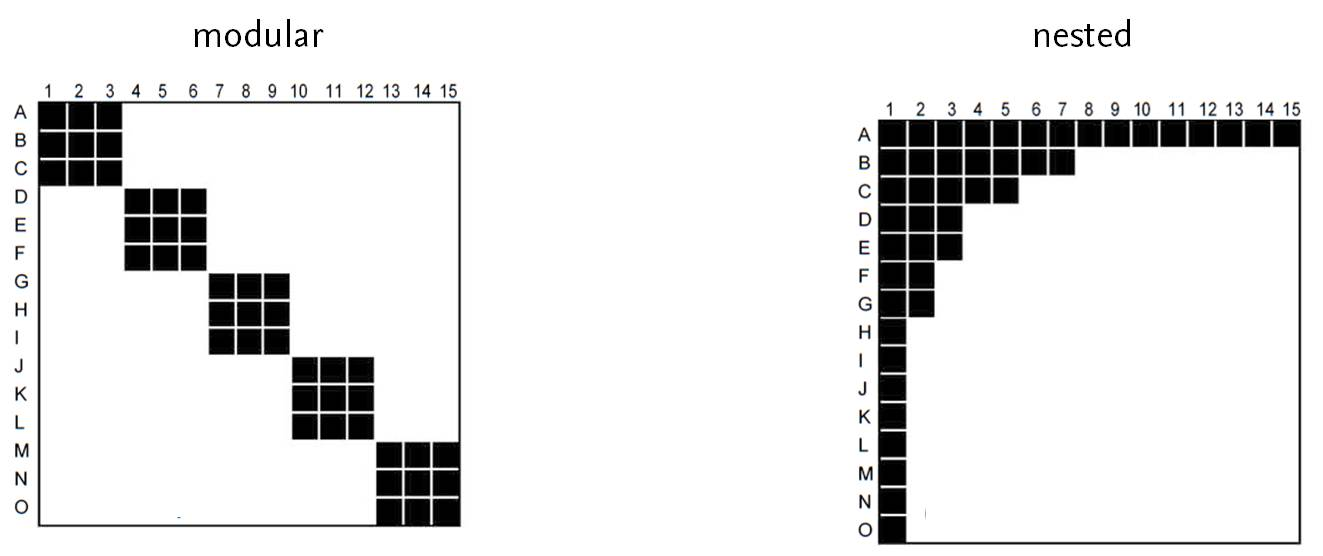
\includegraphics[width=18.38in]{fig06Networks/Lewinsohn}

In the following we will more strongly focus on modularity than on nestedness, for reasons that will be explained later.

\subsection{Modularity}\label{modularity}

Modularity, as defined by Newman, is given by the following formula:
\[\begin{equation}
Q = \frac{1}{A} \sum_{i,j} \left[ a_{ij} - \frac{d_i d_j}{A}\right]\delta_{ij}
\end{equation}\]
where \(A\) is the total number of connections in the network (i.e.~\(A = \sum_i \sum_j a_{ij}\)), \(d_i\) is the degree of species \(i\) (i.e.~\(d_i = \sum_j a_{ij}\)) and the \(\delta_{ij}\) are dummy variables indicating whether species/nodes \(i\) and \(j\) are assumed to belong to the same module/community/cluster.
In layman's terms, modularity is a quantity that measures how ``intense'\,' interactions are within modules, and thus by contrast how little interaction there is between nodes belonging to different modules.
The principle of modularity search is to look for the partitioning of nodes into communities/modules that maximizes the associated modularity score.
The problem of modularity search is quite complex (NP-complete problem) and thus can be solved with different algorithms that have their pros and cons.

Modularity, in its classic form, only works for undirected networks.
Three algorithms that are often used in ecology are the edge-betweenness algorithm (EB), the leading-eigenvector one (LE) and the Louvain algorithm (ML).

\begin{Shaded}
\begin{Highlighting}[]
\NormalTok{net}\OtherTok{\textless{}{-}}\FunctionTok{sample\_gnp}\NormalTok{(}\DecValTok{100}\NormalTok{,}\FloatTok{0.2}\NormalTok{, }\AttributeTok{directed =} \ConstantTok{FALSE}\NormalTok{)}
\NormalTok{EB.mod}\OtherTok{\textless{}{-}}\FunctionTok{cluster\_edge\_betweenness}\NormalTok{(net)}
\NormalTok{LE.mod}\OtherTok{\textless{}{-}}\FunctionTok{cluster\_leading\_eigen}\NormalTok{(net)}
\NormalTok{ML.mod}\OtherTok{\textless{}{-}}\FunctionTok{cluster\_louvain}\NormalTok{(net)}

\FunctionTok{plot}\NormalTok{(EB.mod,net,}\AttributeTok{layout =}\NormalTok{ layout\_with\_mds)}
\end{Highlighting}
\end{Shaded}

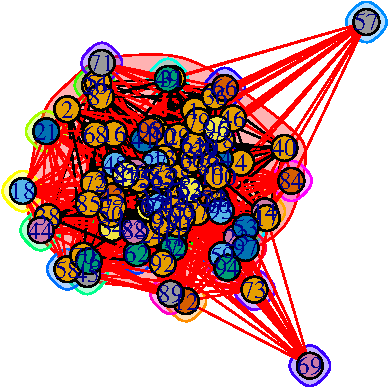
\includegraphics{_main_files/figure-latex/unnamed-chunk-33-1.pdf}

\begin{Shaded}
\begin{Highlighting}[]
\FunctionTok{plot}\NormalTok{(LE.mod,net,}\AttributeTok{layout =}\NormalTok{ layout\_with\_mds)}
\end{Highlighting}
\end{Shaded}

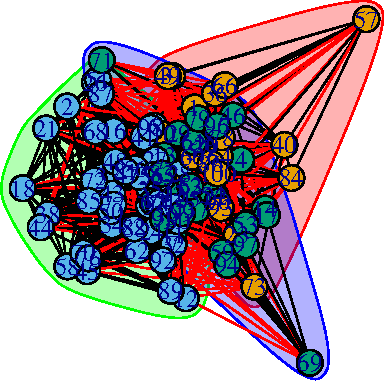
\includegraphics{_main_files/figure-latex/unnamed-chunk-33-2.pdf}

\begin{Shaded}
\begin{Highlighting}[]
\FunctionTok{plot}\NormalTok{(ML.mod,net,}\AttributeTok{layout =}\NormalTok{ layout\_with\_mds)}
\end{Highlighting}
\end{Shaded}

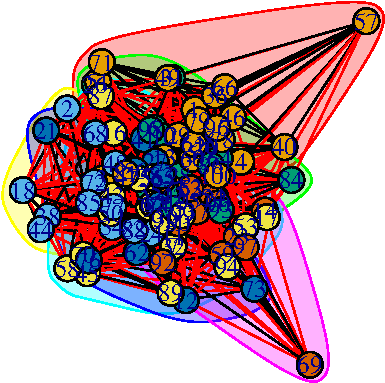
\includegraphics{_main_files/figure-latex/unnamed-chunk-33-3.pdf}

Again, modularity is not adapted to directed networks, but there ways to circumvent this issue:
- by making the network/adjacency matrix symmetric
- through the use of another definition of modularity (e.g.~the infomap definition of Rosvall and Bergström)

\subsubsection{Modularity of the empirical food web}\label{modularity-of-the-empirical-food-web}

As mentioned before, it is highly recommended to check whether the obtained modularity is ``expected'\,' or extraordinary using a null model. Here is an example using the empirical food web.

\begin{Shaded}
\begin{Highlighting}[]
\NormalTok{modul}\OtherTok{\textless{}{-}}\FunctionTok{cluster\_louvain}\NormalTok{(}\FunctionTok{graph\_from\_adjacency\_matrix}\NormalTok{(mat,}\AttributeTok{mode=}\StringTok{"undirected"}\NormalTok{))}
\end{Highlighting}
\end{Shaded}

\begin{verbatim}
## Warning: The `adjmatrix` argument of `graph_from_adjacency_matrix()` must be symmetric
## with mode = "undirected" as of igraph 1.6.0.
## i Use mode = "max" to achieve the original behavior.
## This warning is displayed once every 8 hours.
## Call `lifecycle::last_lifecycle_warnings()` to see where this warning was
## generated.
\end{verbatim}

\begin{Shaded}
\begin{Highlighting}[]
\NormalTok{moduls}\OtherTok{\textless{}{-}}\FunctionTok{lapply}\NormalTok{(}\DecValTok{1}\SpecialCharTok{:}\DecValTok{100}\NormalTok{,}\ControlFlowTok{function}\NormalTok{(x) }\FunctionTok{cluster\_louvain}\NormalTok{(}\FunctionTok{graph\_from\_adjacency\_matrix}\NormalTok{(ms[[x]],}\AttributeTok{mode=}\StringTok{"undirected"}\NormalTok{))}\SpecialCharTok{$}\NormalTok{modularity)}
\FunctionTok{plot}\NormalTok{(}\FunctionTok{density}\NormalTok{(}\FunctionTok{unlist}\NormalTok{(moduls)))}
\end{Highlighting}
\end{Shaded}

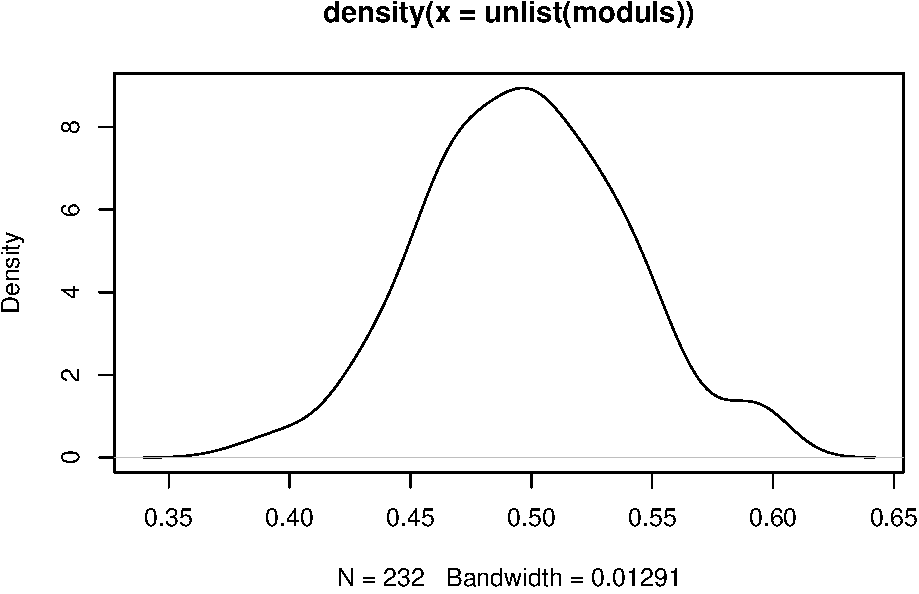
\includegraphics{_main_files/figure-latex/unnamed-chunk-34-1.pdf}

\begin{Shaded}
\begin{Highlighting}[]
\NormalTok{modul.ecdf}\OtherTok{\textless{}{-}}\FunctionTok{ecdf}\NormalTok{(}\FunctionTok{unlist}\NormalTok{(moduls))}
\DecValTok{1}\SpecialCharTok{{-}}\FunctionTok{modul.ecdf}\NormalTok{(modul}\SpecialCharTok{$}\NormalTok{modularity[}\DecValTok{2}\NormalTok{])}
\end{Highlighting}
\end{Shaded}

\begin{verbatim}
## [1] 1
\end{verbatim}

\subsubsection{Which algorithm?}\label{which-algorithm}

Because there are tons of algorithms already developed to find clusters/communities/modules in networks, it is easy to get lost\ldots{} Yet two papers (at least) have made our life easier by comparing all these algorithms, bot for unipartite networks (Yang et al.~2016) and bipartite networks (Leger et al.~2015).

\subsection{Block models}\label{block-models}

Another possibility when looking for clusters of species that interact more among themselves is to look for blocks of nodes/species that ``behave'\,' similarly. This can be achieved using stochastic block models (SBM), also sometimes called latent block models (LBM) when dealing with bipartite networks.

Block models work by optimizing the fit of a model (in the classic statistical sense) which assigns probability of membership to groups and probability of interaction between nodes of known groups.
Block models can be fitted on different kinds of adjacency matrices following different distributions (e.g.~Bernoulli for binary adjacency matrices, Poisson for counts, etc.).
The inference of a block model yields one parameter per block (the ``expected connection'\,' within the block) and the proportions of nodes belonging to each group.

\begin{Shaded}
\begin{Highlighting}[]
\NormalTok{sbmnet }\OtherTok{\textless{}{-}} \FunctionTok{sampleSimpleSBM}\NormalTok{(}\DecValTok{100}\NormalTok{, }\FunctionTok{c}\NormalTok{(.}\DecValTok{5}\NormalTok{, .}\DecValTok{25}\NormalTok{, .}\DecValTok{25}\NormalTok{), }\FunctionTok{list}\NormalTok{(}\AttributeTok{mean =} \FunctionTok{diag}\NormalTok{(.}\DecValTok{4}\NormalTok{, }\DecValTok{3}\NormalTok{) }\SpecialCharTok{+} \FloatTok{0.05}\NormalTok{), }\AttributeTok{model =} \StringTok{\textquotesingle{}bernoulli\textquotesingle{}}\NormalTok{)}
\FunctionTok{head}\NormalTok{(sbmnet}\SpecialCharTok{$}\NormalTok{networkData)}
\end{Highlighting}
\end{Shaded}

\begin{verbatim}
##      [,1] [,2] [,3] [,4] [,5] [,6] [,7] [,8] [,9] [,10] [,11] [,12] [,13] [,14]
## [1,]   NA    0    0    0    0    0    1    0    0     0     1     0     1     0
## [2,]    0   NA    0    0    0    0    1    0    0     0     0     0     0     0
## [3,]    0    0   NA    0    0    0    0    0    0     1     0     0     0     0
## [4,]    0    0    0   NA    1    0    0    1    0     0     0     0     0     0
## [5,]    0    0    0    1   NA    1    1    0    0     0     0     0     0     0
## [6,]    0    0    0    0    1   NA    0    0    1     0     0     0     0     0
##      [,15] [,16] [,17] [,18] [,19] [,20] [,21] [,22] [,23] [,24] [,25] [,26]
## [1,]     0     0     0     1     0     0     0     0     0     0     0     0
## [2,]     0     0     0     0     0     0     0     0     1     0     0     0
## [3,]     0     0     0     0     0     0     0     1     0     0     0     0
## [4,]     1     0     0     0     0     0     0     0     1     0     1     0
## [5,]     0     0     0     0     0     0     1     0     0     0     0     0
## [6,]     0     0     0     0     0     0     1     1     0     0     0     0
##      [,27] [,28] [,29] [,30] [,31] [,32] [,33] [,34] [,35] [,36] [,37] [,38]
## [1,]     1     0     0     0     0     1     0     0     1     0     0     0
## [2,]     0     0     0     0     0     0     0     0     0     0     0     0
## [3,]     0     0     0     0     0     1     0     0     0     0     0     0
## [4,]     0     0     0     0     0     1     0     0     0     0     0     0
## [5,]     0     1     0     1     0     0     0     0     0     0     1     0
## [6,]     0     1     0     1     0     0     0     0     0     1     1     0
##      [,39] [,40] [,41] [,42] [,43] [,44] [,45] [,46] [,47] [,48] [,49] [,50]
## [1,]     0     0     0     0     0     0     1     0     0     0     0     0
## [2,]     0     0     0     0     1     0     0     0     0     0     0     0
## [3,]     1     0     0     0     0     0     0     0     0     0     0     0
## [4,]     0     0     0     0     1     0     0     0     0     0     1     1
## [5,]     0     0     1     1     0     0     0     0     0     0     0     0
## [6,]     0     1     0     0     0     0     0     0     0     0     1     0
##      [,51] [,52] [,53] [,54] [,55] [,56] [,57] [,58] [,59] [,60] [,61] [,62]
## [1,]     0     0     0     1     0     0     0     0     0     0     0     0
## [2,]     1     0     0     0     0     0     0     1     1     0     0     1
## [3,]     0     0     0     1     1     0     0     0     0     0     0     0
## [4,]     0     0     0     1     0     0     0     0     0     0     0     1
## [5,]     0     0     0     0     0     0     0     0     1     0     1     1
## [6,]     0     0     0     0     0     1     0     0     1     0     0     0
##      [,63] [,64] [,65] [,66] [,67] [,68] [,69] [,70] [,71] [,72] [,73] [,74]
## [1,]     0     0     0     0     0     0     0     0     0     1     0     0
## [2,]     0     0     0     0     0     0     0     1     0     0     1     0
## [3,]     0     0     0     1     0     0     0     0     0     1     0     0
## [4,]     0     0     0     0     1     0     0     0     0     0     1     0
## [5,]     0     0     0     0     1     0     0     0     0     0     0     0
## [6,]     0     0     0     1     1     0     0     0     1     0     0     0
##      [,75] [,76] [,77] [,78] [,79] [,80] [,81] [,82] [,83] [,84] [,85] [,86]
## [1,]     0     0     0     1     0     1     0     0     0     1     0     0
## [2,]     1     0     0     0     0     0     0     0     0     0     1     0
## [3,]     0     0     0     1     0     0     0     0     0     1     0     0
## [4,]     0     0     0     0     0     0     0     0     0     0     0     0
## [5,]     0     0     0     0     0     0     1     0     0     0     0     1
## [6,]     0     0     0     0     0     0     1     0     0     1     0     0
##      [,87] [,88] [,89] [,90] [,91] [,92] [,93] [,94] [,95] [,96] [,97] [,98]
## [1,]     0     0     0     0     0     0     0     0     0     0     0     0
## [2,]     0     0     0     0     0     0     0     0     0     1     1     0
## [3,]     0     0     0     0     1     0     0     0     0     1     1     0
## [4,]     0     0     0     0     0     0     0     0     0     0     0     1
## [5,]     0     0     0     0     0     0     0     0     0     0     0     1
## [6,]     0     0     0     0     0     0     1     0     1     0     0     1
##      [,99] [,100]
## [1,]     0      1
## [2,]     0      0
## [3,]     0      0
## [4,]     0      0
## [5,]     0      0
## [6,]     0      0
\end{verbatim}

\begin{Shaded}
\begin{Highlighting}[]
\NormalTok{net.SBM }\OtherTok{\textless{}{-}} \FunctionTok{estimateSimpleSBM}\NormalTok{(}\FunctionTok{as.matrix}\NormalTok{(sbmnet}\SpecialCharTok{$}\NormalTok{networkData))}
\end{Highlighting}
\end{Shaded}

\begin{verbatim}
## -> Estimation for 1 groups
## 
\end{verbatim}

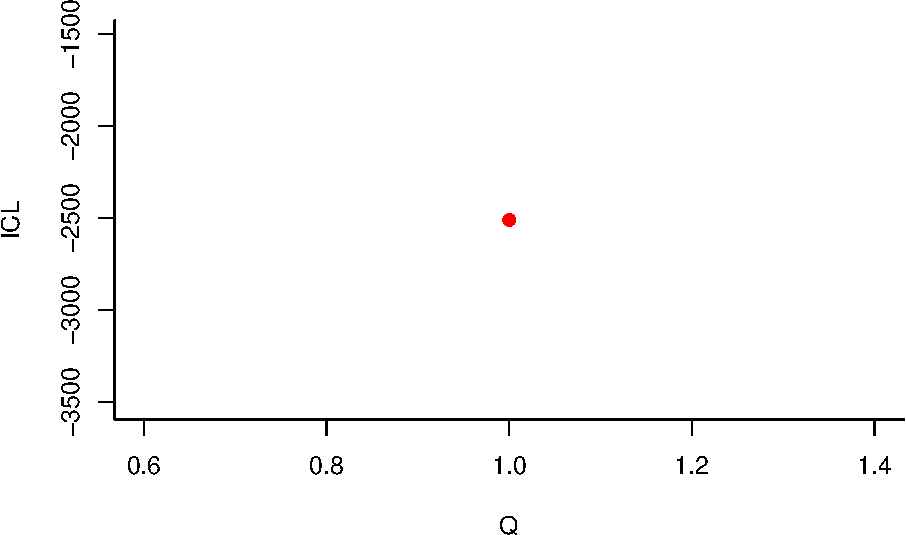
\includegraphics{_main_files/figure-latex/unnamed-chunk-35-1.pdf}

\begin{verbatim}
## -> Computation of eigen decomposition used for initalizations
## 
## -> Pass 1
##     -> With ascending number of groups
##         -> For 2 groups
## 
\end{verbatim}

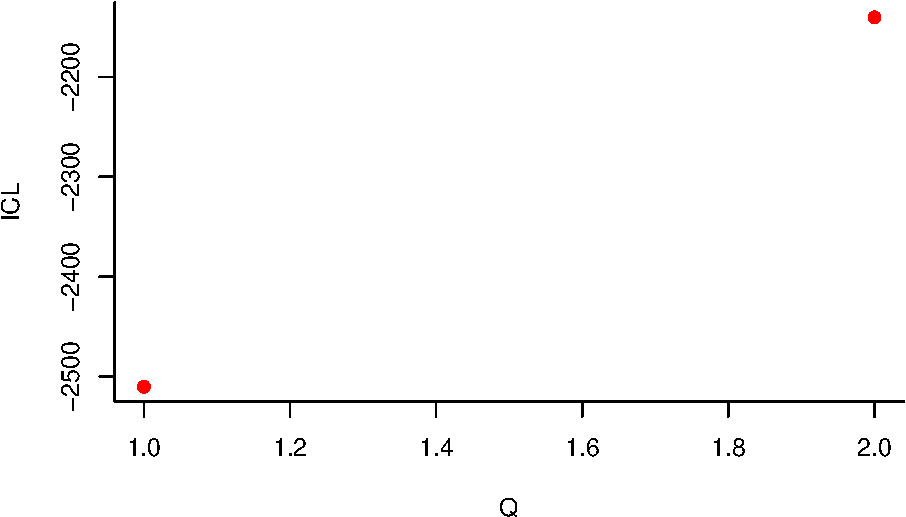
\includegraphics{_main_files/figure-latex/unnamed-chunk-35-2.pdf}

\begin{verbatim}
##         -> For 3 groups
## 
\end{verbatim}

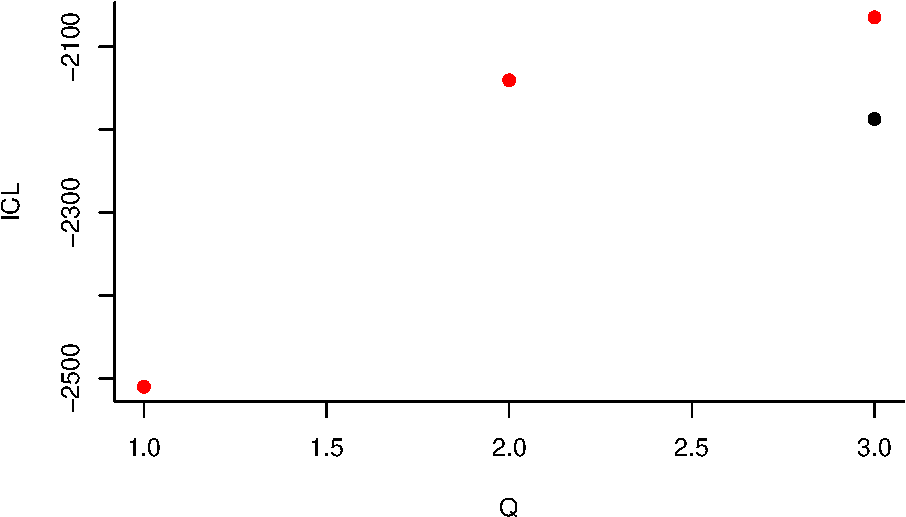
\includegraphics{_main_files/figure-latex/unnamed-chunk-35-3.pdf}

\begin{verbatim}
##         -> For 4 groups
## 
\end{verbatim}

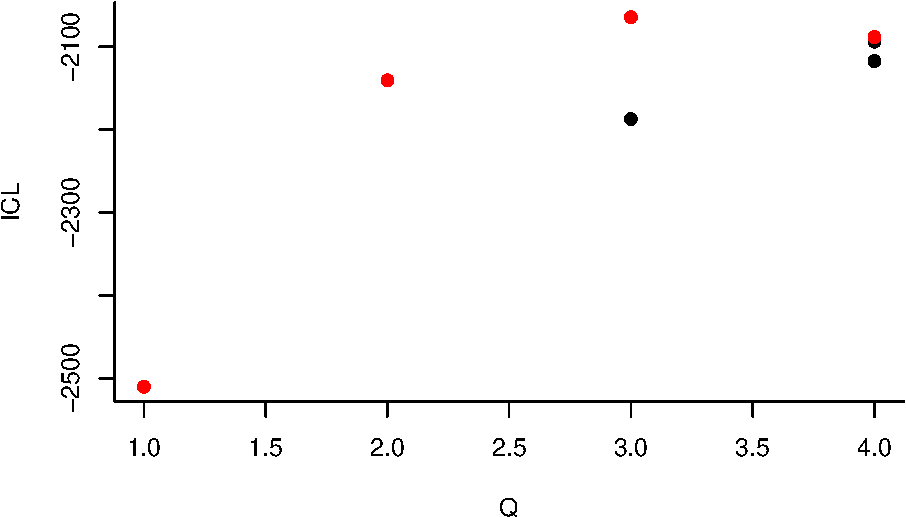
\includegraphics{_main_files/figure-latex/unnamed-chunk-35-4.pdf}

\begin{verbatim}
##         -> For 5 groups
## 
\end{verbatim}

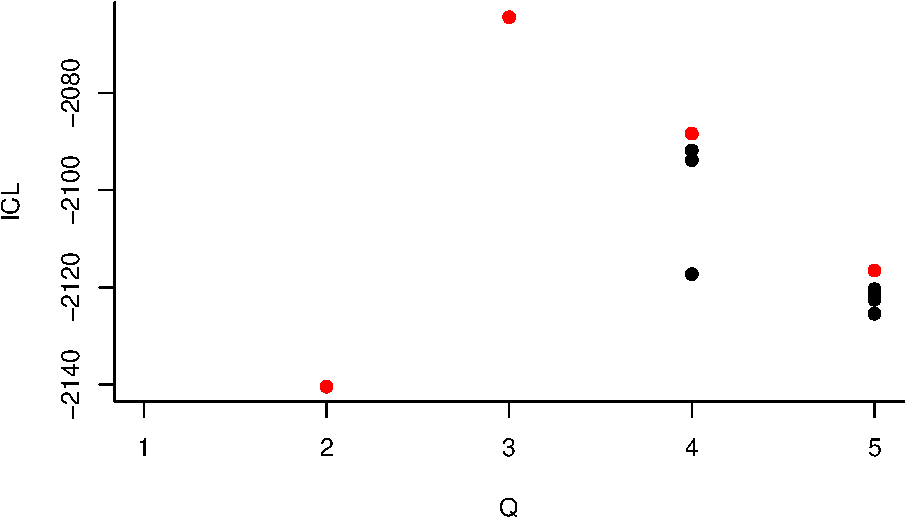
\includegraphics{_main_files/figure-latex/unnamed-chunk-35-5.pdf}

\begin{verbatim}
##     -> With descending number of groups
##         -> For 4 groups
## 
\end{verbatim}

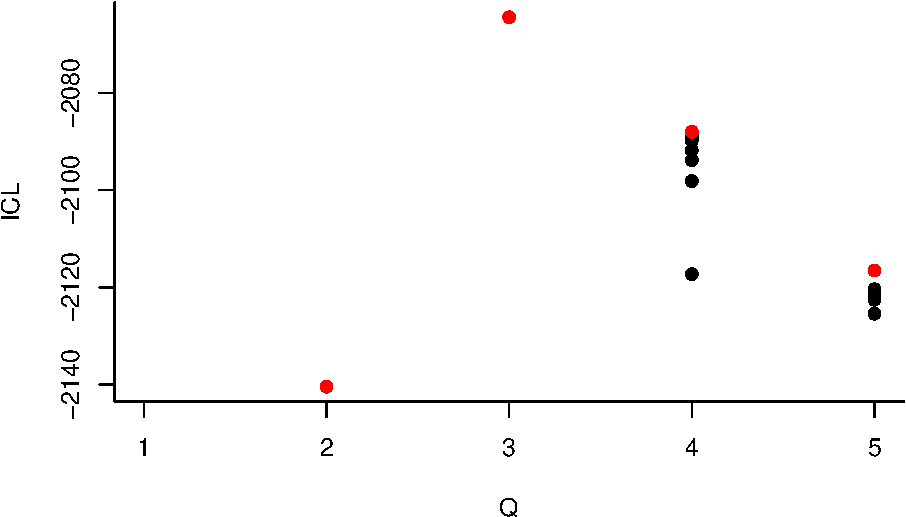
\includegraphics{_main_files/figure-latex/unnamed-chunk-35-6.pdf}

\begin{verbatim}
##         -> For 3 groups
## 
\end{verbatim}

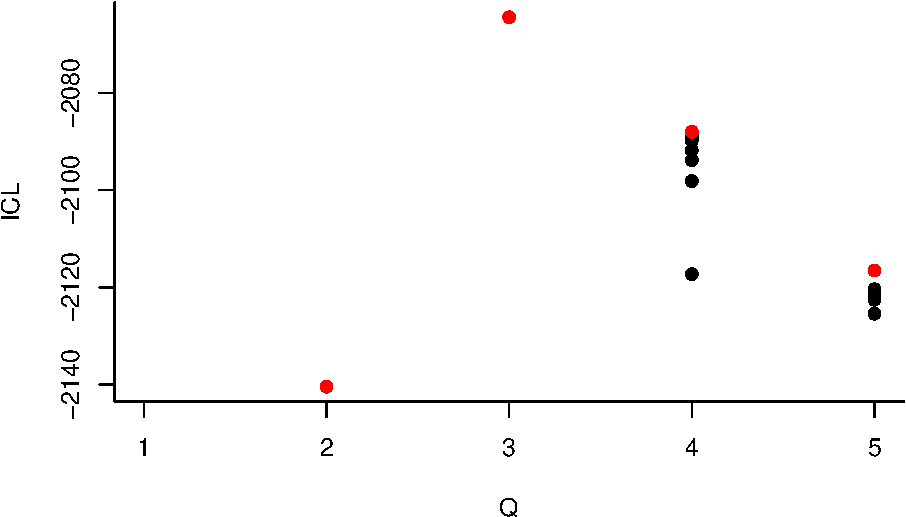
\includegraphics{_main_files/figure-latex/unnamed-chunk-35-7.pdf}

\begin{verbatim}
##         -> For 2 groups
## 
\end{verbatim}

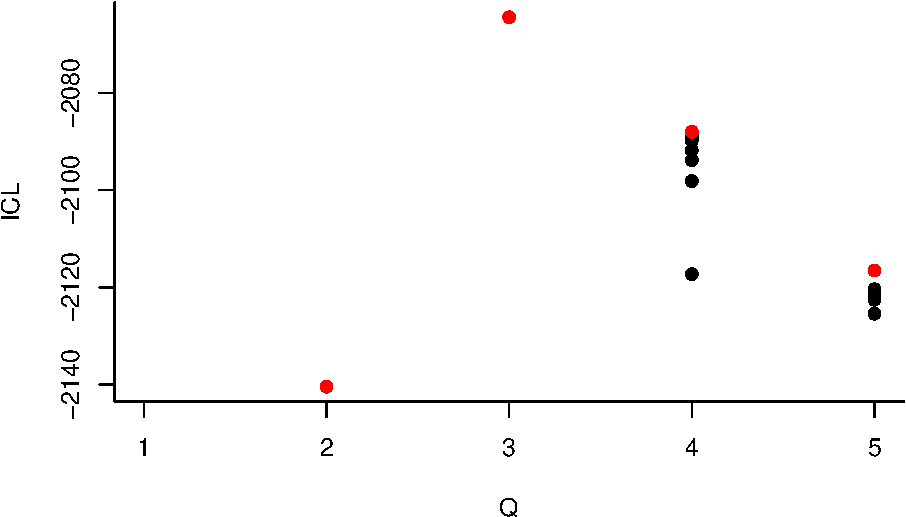
\includegraphics{_main_files/figure-latex/unnamed-chunk-35-8.pdf}

\begin{verbatim}
## -> Pass 2
##     -> With ascending number of groups
##         -> For 2 groups
##         -> For 3 groups
##         -> For 4 groups
##         -> For 5 groups
## 
\end{verbatim}

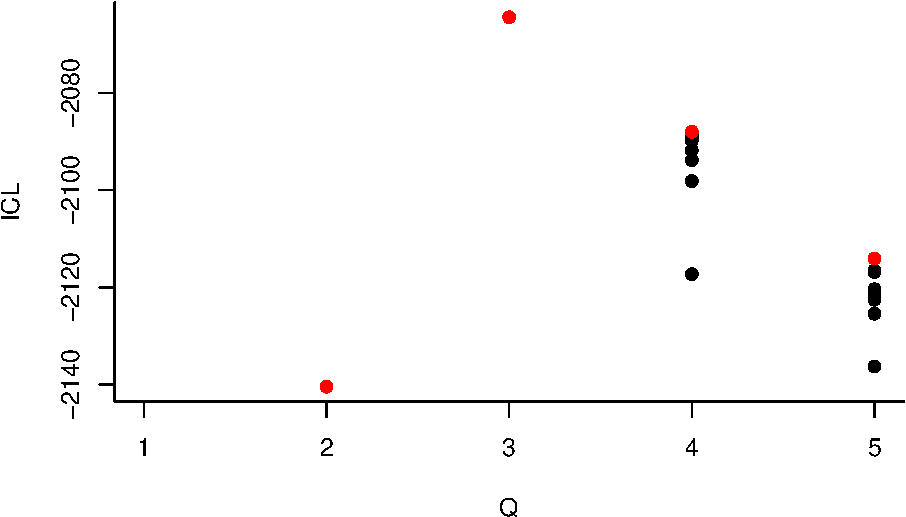
\includegraphics{_main_files/figure-latex/unnamed-chunk-35-9.pdf}

\begin{verbatim}
##     -> With descending number of groups
##         -> For 4 groups
## 
\end{verbatim}

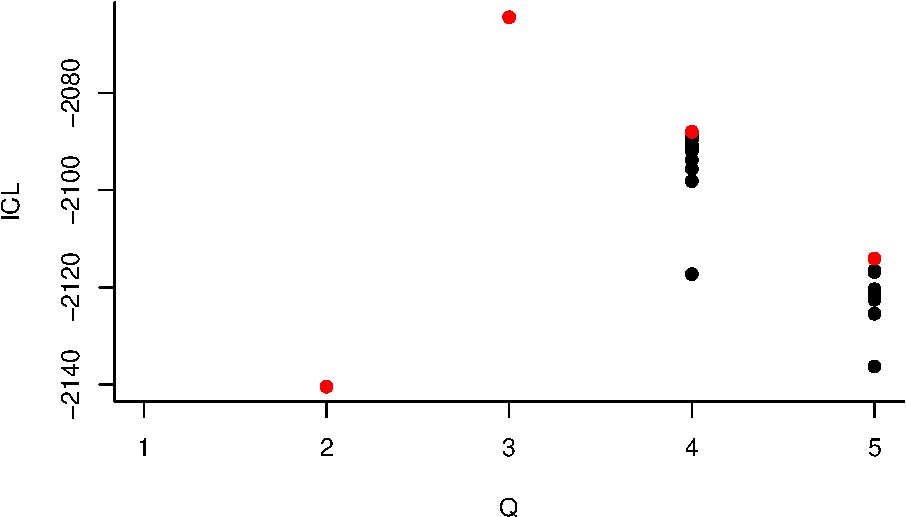
\includegraphics{_main_files/figure-latex/unnamed-chunk-35-10.pdf}

\begin{verbatim}
##         -> For 3 groups
##         -> For 2 groups
## -> Pass 3
##     -> With ascending number of groups
##         -> For 2 groups
##         -> For 3 groups
##         -> For 4 groups
##         -> For 5 groups
##     -> With descending number of groups
##         -> For 4 groups
##         -> For 3 groups
##         -> For 2 groups
\end{verbatim}

\begin{Shaded}
\begin{Highlighting}[]
\FunctionTok{plot}\NormalTok{(net.SBM, }\StringTok{\textquotesingle{}expected\textquotesingle{}}\NormalTok{)}
\end{Highlighting}
\end{Shaded}

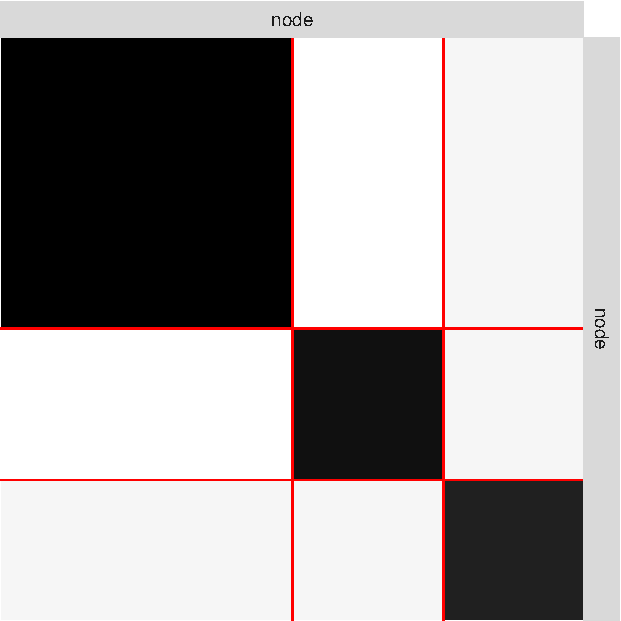
\includegraphics{_main_files/figure-latex/unnamed-chunk-35-11.pdf}

\begin{Shaded}
\begin{Highlighting}[]
\FunctionTok{plot}\NormalTok{(net.SBM, }\StringTok{\textquotesingle{}data\textquotesingle{}}\NormalTok{)}
\end{Highlighting}
\end{Shaded}

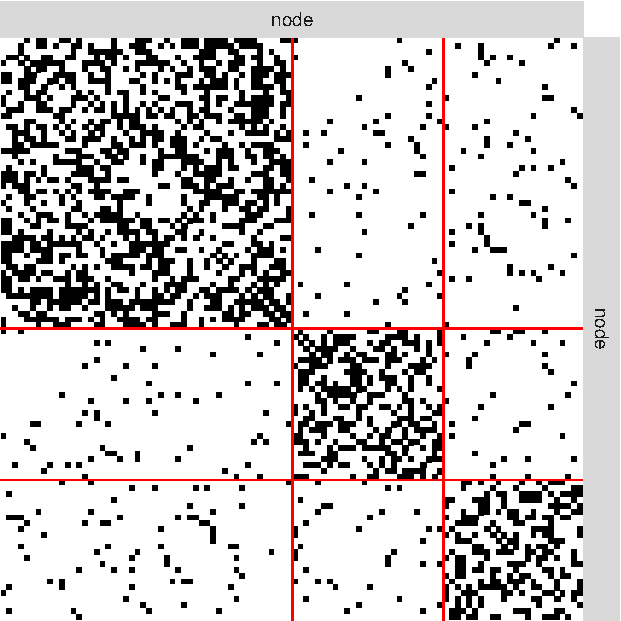
\includegraphics{_main_files/figure-latex/unnamed-chunk-35-12.pdf}

\subsection{Modularity and blocks}\label{modularity-and-blocks}

It is possible to compare the partitionings of nodes obtained through modularity search and SBMs, for instance comparing the result of Louvain algorithm with a simple SBM on the network given by mat.

The alluvial plot helps visualize the correspondence between these groups.

\begin{Shaded}
\begin{Highlighting}[]
\NormalTok{m.SBM }\OtherTok{\textless{}{-}} \FunctionTok{estimateSimpleSBM}\NormalTok{(mat)}
\end{Highlighting}
\end{Shaded}

\begin{verbatim}
## -> Estimation for 1 groups
## 
\end{verbatim}

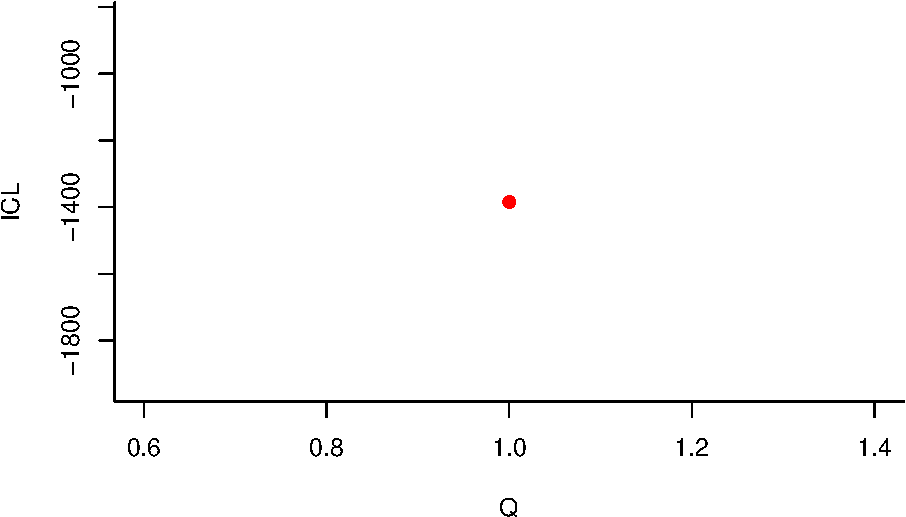
\includegraphics{_main_files/figure-latex/unnamed-chunk-36-1.pdf}

\begin{verbatim}
## -> Computation of eigen decomposition used for initalizations
## 
## -> Pass 1
##     -> With ascending number of groups
##         -> For 2 groups
## 
\end{verbatim}

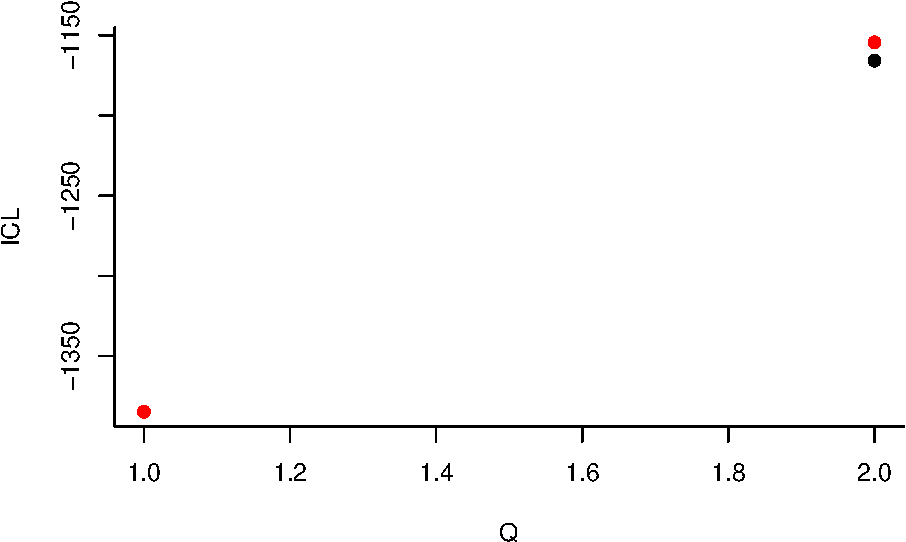
\includegraphics{_main_files/figure-latex/unnamed-chunk-36-2.pdf}

\begin{verbatim}
##         -> For 3 groups
## 
\end{verbatim}

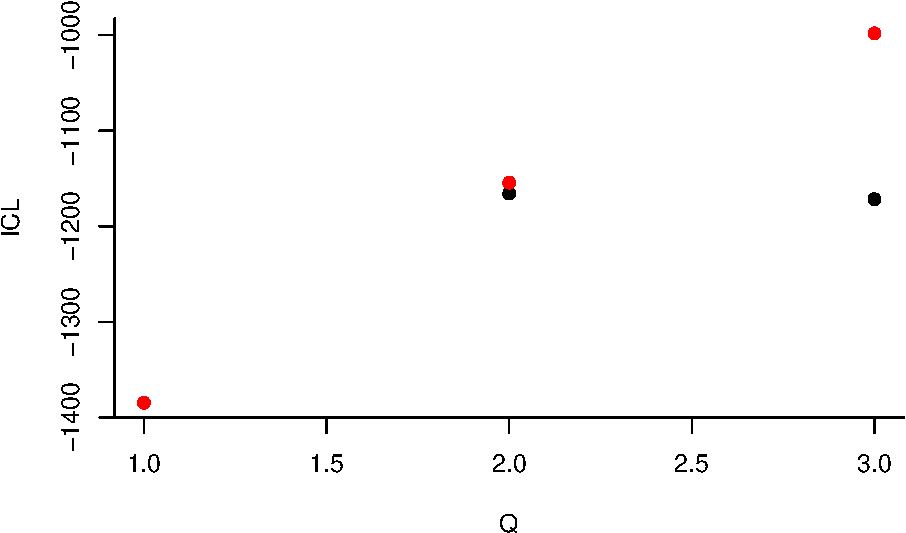
\includegraphics{_main_files/figure-latex/unnamed-chunk-36-3.pdf}

\begin{verbatim}
##         -> For 4 groups
## 
\end{verbatim}

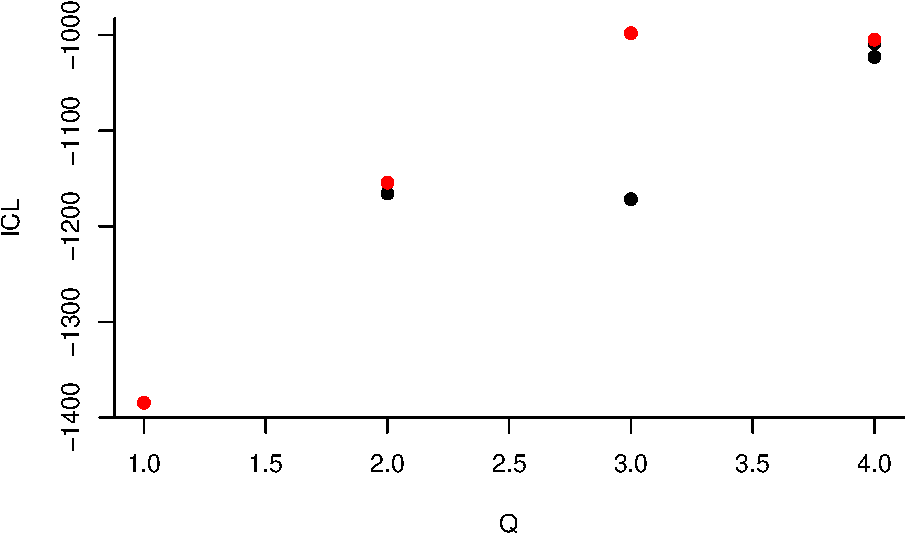
\includegraphics{_main_files/figure-latex/unnamed-chunk-36-4.pdf}

\begin{verbatim}
##         -> For 5 groups
## 
\end{verbatim}

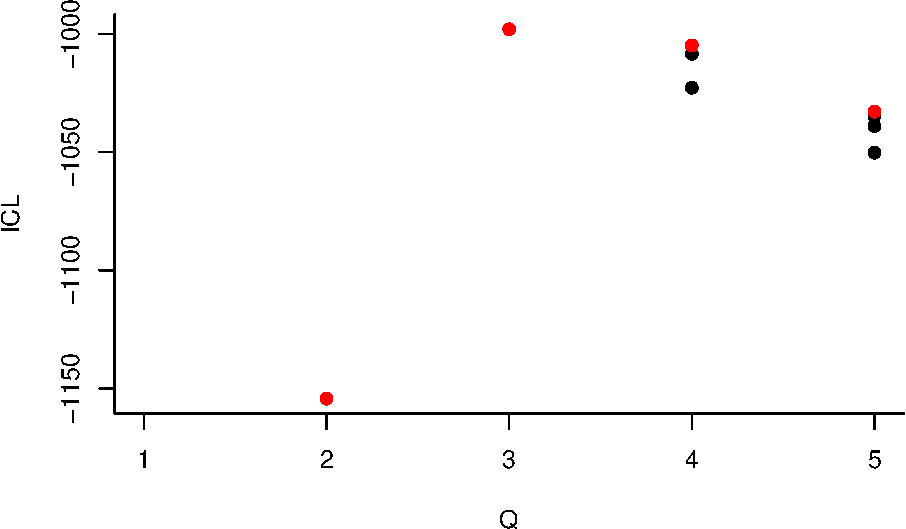
\includegraphics{_main_files/figure-latex/unnamed-chunk-36-5.pdf}

\begin{verbatim}
##     -> With descending number of groups
##         -> For 4 groups
## 
\end{verbatim}

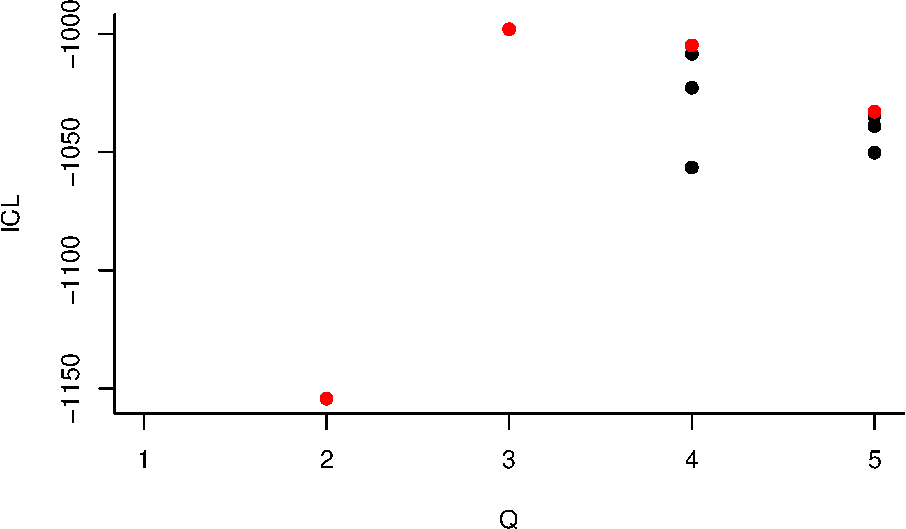
\includegraphics{_main_files/figure-latex/unnamed-chunk-36-6.pdf}

\begin{verbatim}
##         -> For 3 groups
## 
\end{verbatim}

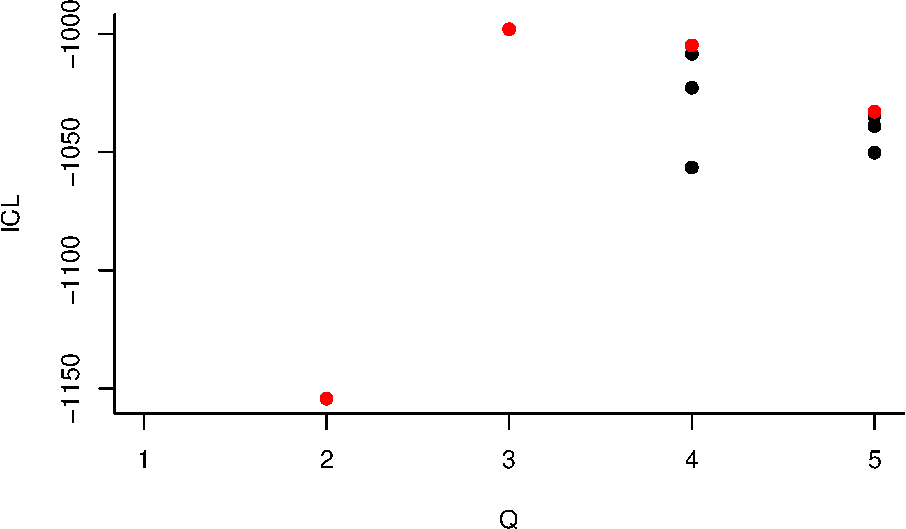
\includegraphics{_main_files/figure-latex/unnamed-chunk-36-7.pdf}

\begin{verbatim}
##         -> For 2 groups
## 
\end{verbatim}

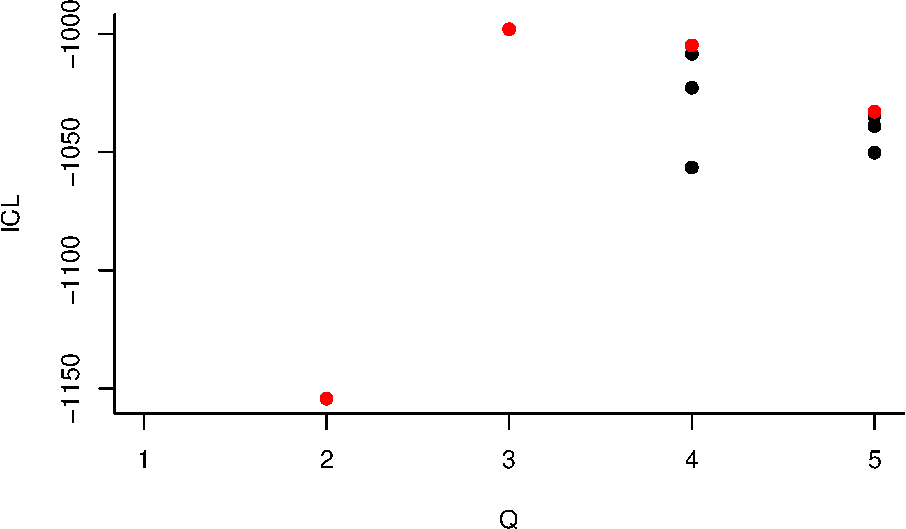
\includegraphics{_main_files/figure-latex/unnamed-chunk-36-8.pdf}

\begin{verbatim}
## -> Pass 2
##     -> With ascending number of groups
##         -> For 2 groups
##         -> For 3 groups
##         -> For 4 groups
##         -> For 5 groups
##     -> With descending number of groups
##         -> For 4 groups
##         -> For 3 groups
##         -> For 2 groups
\end{verbatim}

\begin{Shaded}
\begin{Highlighting}[]
\NormalTok{modul}\OtherTok{\textless{}{-}}\FunctionTok{cluster\_louvain}\NormalTok{(}\FunctionTok{graph\_from\_adjacency\_matrix}\NormalTok{(mat,}\AttributeTok{mode=}\StringTok{"undirected"}\NormalTok{))}
\FunctionTok{make\_alluvial\_2}\NormalTok{(m.SBM}\SpecialCharTok{$}\NormalTok{memberships,modul}\SpecialCharTok{$}\NormalTok{membership,}\StringTok{"Blocks"}\NormalTok{,}\StringTok{"Modules"}\NormalTok{)}
\end{Highlighting}
\end{Shaded}

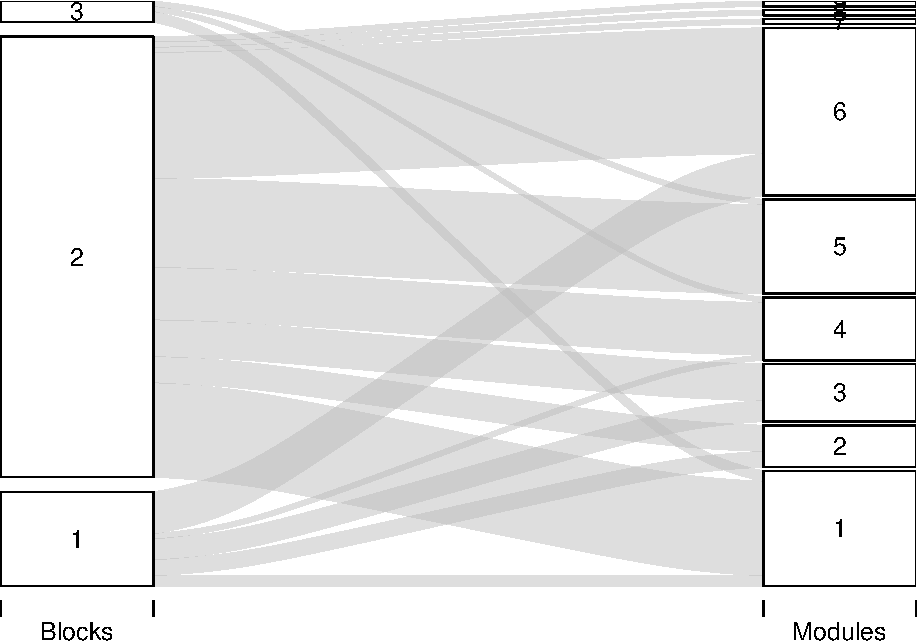
\includegraphics{_main_files/figure-latex/unnamed-chunk-36-9.pdf}

It is also possible to look at whether these groupings have anything to do with trophic level (sensus MacKay et al.).

\begin{Shaded}
\begin{Highlighting}[]
\FunctionTok{count\_components}\NormalTok{(net.mat)}
\end{Highlighting}
\end{Shaded}

\begin{verbatim}
## [1] 4
\end{verbatim}

\begin{Shaded}
\begin{Highlighting}[]
\NormalTok{net.comp}\OtherTok{\textless{}{-}}\FunctionTok{components}\NormalTok{(net.mat)}
\NormalTok{tl}\FloatTok{.1}\OtherTok{\textless{}{-}}\FunctionTok{trophic\_levels}\NormalTok{(}\FunctionTok{largest\_component}\NormalTok{(net.mat))}
\FunctionTok{plot}\NormalTok{(}\FunctionTok{largest\_component}\NormalTok{(net.mat),}\AttributeTok{layout =}\NormalTok{ layout\_as\_food\_web)}
\end{Highlighting}
\end{Shaded}

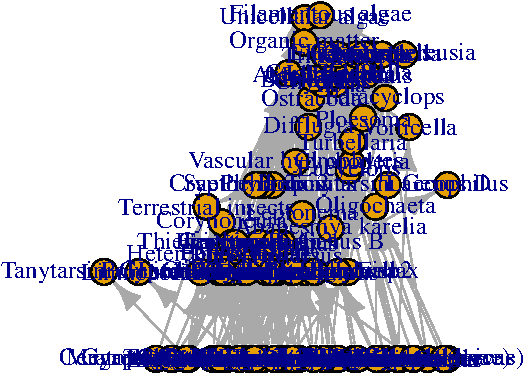
\includegraphics{_main_files/figure-latex/unnamed-chunk-37-1.pdf}

\begin{Shaded}
\begin{Highlighting}[]
\FunctionTok{plot}\NormalTok{(tl}\FloatTok{.1}\SpecialCharTok{\textasciitilde{}}\FunctionTok{as.factor}\NormalTok{(m.SBM}\SpecialCharTok{$}\NormalTok{indMemberships[}\FunctionTok{which}\NormalTok{(net.comp}\SpecialCharTok{$}\NormalTok{membership}\SpecialCharTok{==}\DecValTok{1}\NormalTok{),]}\SpecialCharTok{\%*\%}\NormalTok{(}\DecValTok{1}\SpecialCharTok{:}\DecValTok{3}\NormalTok{)),}\AttributeTok{xlab=}\StringTok{"SBM group"}\NormalTok{,}\AttributeTok{ylab=}\StringTok{"Trophic level"}\NormalTok{)}
\end{Highlighting}
\end{Shaded}

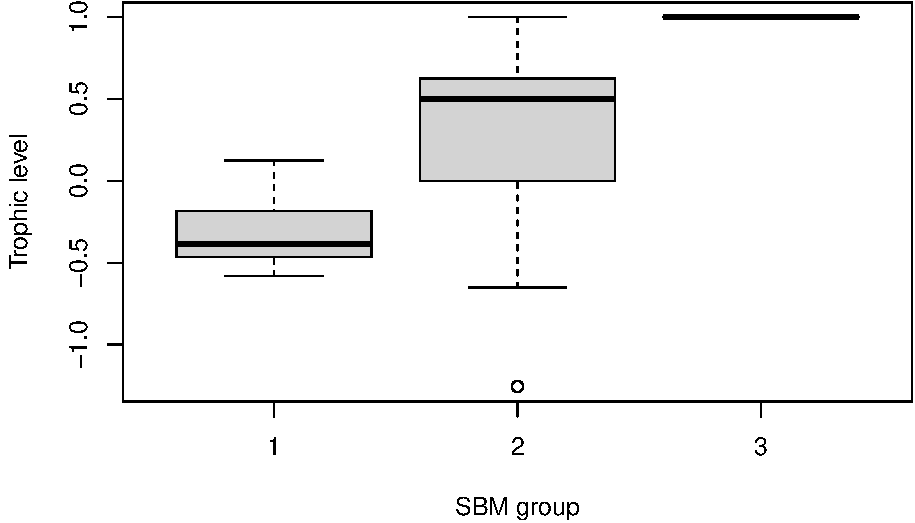
\includegraphics{_main_files/figure-latex/unnamed-chunk-37-2.pdf}

\begin{Shaded}
\begin{Highlighting}[]
\FunctionTok{plot}\NormalTok{(tl}\FloatTok{.1}\SpecialCharTok{\textasciitilde{}}\FunctionTok{as.factor}\NormalTok{(modul}\SpecialCharTok{$}\NormalTok{membership[}\FunctionTok{which}\NormalTok{(net.comp}\SpecialCharTok{$}\NormalTok{membership}\SpecialCharTok{==}\DecValTok{1}\NormalTok{)]),}\AttributeTok{xlab=}\StringTok{"module"}\NormalTok{,}\AttributeTok{ylab=}\StringTok{"Trophic level"}\NormalTok{)}
\end{Highlighting}
\end{Shaded}

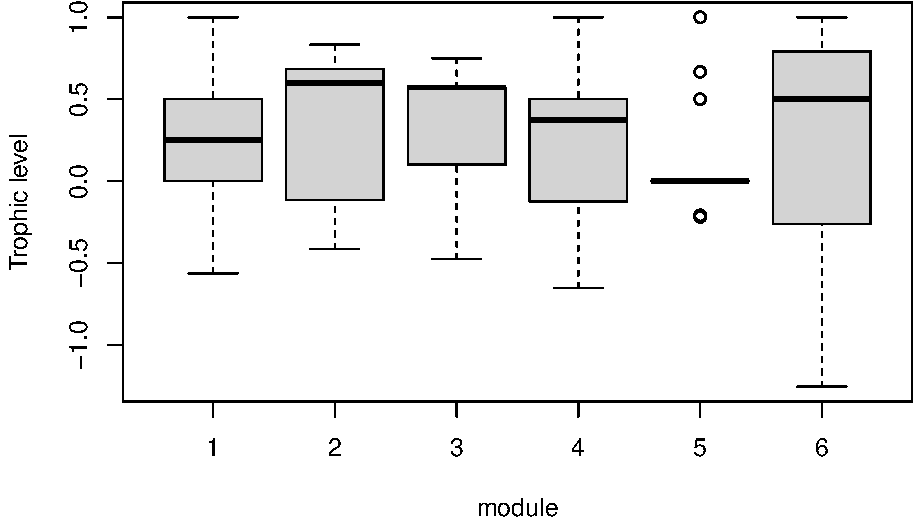
\includegraphics{_main_files/figure-latex/unnamed-chunk-37-3.pdf}

As we can see, SBM-derived groups seem to be better at capturing trophic levels.

\subsection{Spectral clustering}\label{spectral-clustering}

One drawback of SBM is that they can be slow to converge, especially when the dataset is big. A convenient replacement algorithm when the number of groups to look for is known (or can be easily guessed) is spectral clustering.
The idea of spectral clustering is to make use of the Laplacian matrix \(L\) of the graph, given by:
\[L = D - A\]
where \(D\) is the diagonal matrix of nodes' degrees and \(A\) is the adjacency matrix.

The Laplacian matrix has interesting properties, the best of all being that the number of zeros among its eigenvalues yield the number of components of the graph (one 0 means there is a single connected component, two zeros means the network is split in two disconnected components, etc.). The eigenvectors associated the zero eigenvalues can inform on the membership of nodes to the different components.

The heuristics of the spectral clustering is to use the eigenvectors associated with the set of small non-zero eigenvalues of \(L\) to deduce the ``almost components'\,' of the graph. To do so, one chooses a number of no-zero eigenvalues to keep and then the algorithm uses the associated eigenvector to find the groups through a K-means algorithm on the space obtained with these eigenvectors.

Here is an example of spectral clustering on the previous block-model graph.

\begin{Shaded}
\begin{Highlighting}[]
\NormalTok{SC}\OtherTok{\textless{}{-}}\FunctionTok{spectral\_clustering}\NormalTok{(}\FunctionTok{graph\_from\_adjacency\_matrix}\NormalTok{(sbmnet}\SpecialCharTok{$}\NormalTok{networkData),}\DecValTok{3}\NormalTok{)}
\FunctionTok{plotMyMatrix}\NormalTok{(sbmnet}\SpecialCharTok{$}\NormalTok{networkData,}\AttributeTok{clustering=}\FunctionTok{list}\NormalTok{(}\StringTok{"row"}\OtherTok{=}\NormalTok{SC,}\StringTok{"col"}\OtherTok{=}\NormalTok{SC))}
\end{Highlighting}
\end{Shaded}

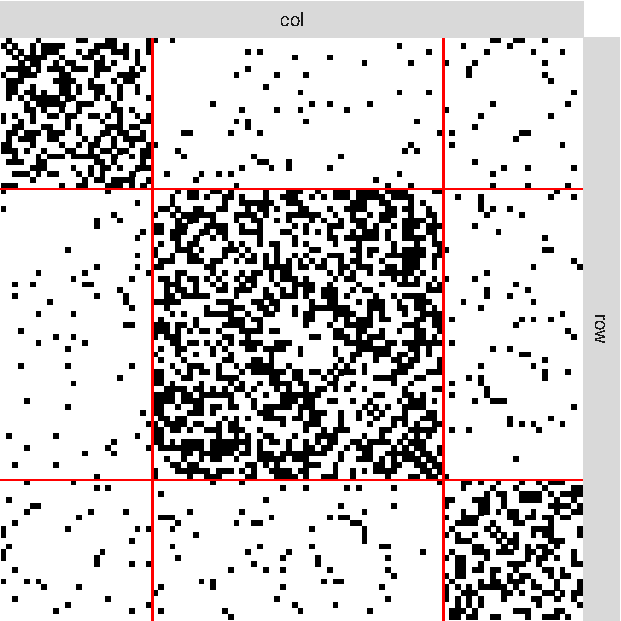
\includegraphics{_main_files/figure-latex/unnamed-chunk-38-1.pdf}

\subsection{Nestedness}\label{nestedness}

The idea of nestedness is to measure the tendency for specialists to only interact with a subsample of the interactors of generalists. In other words, a network would be said ``non-nested'\,' only when specialists would interact more likely with specialists than with generalists.

Several indices have been developed over the years. Navigating their complexity is the purpose of the synthesis written by Podani and Schmera (2012).

I will not delve too long on the topic of nestedness because recent research seem to indicate that the concept is not really fruitful for a variety of reasons:
- it seems to be very strongly linked to connectance
- the diversity of nestedness indices tend to obfuscate its meaning (results reported show more about the index than about the concept)
- these different indices can yield very different results when applied to the same dataset
- in the classic case of power law distributions of degrees, the nestedness scores tend to be completely detrmined by the exponent of the power law
- finally, when putting the common datasets in the right matrix ensemble (i.e.~using correct null models to sample similar matrices), reported nestedness values seem to be completely expected.

\subsection{Last words}\label{last-words}

\begin{itemize}
\tightlist
\item
  ecological interaction networks can be used to study community or ecosystem properties
\item
  random network models can help gauge generalities and specificities of networks
\item
  all network patterns do not have a mechanistic model-based explanation yet, but some do (like the link between feasibility, stability, or robustness and connectance)
\item
  interaction network data of different types lend themselves to different analyses (e.g.~modularity for binary networks, value adjacency matrix with signed interactions for May-like analyses)
\end{itemize}

\section{Literature}\label{literature}

Astegiano, J., Guimarães Jr, P. R., Cheptou, P.-O., Vidal, M. M., Mandai, C. Y., Ashworth, L. \& Massol, F. (2015) Persistence of plants and pollinators in the face of habitat loss: Insights from trait-based metacommunity models. Advances in Ecological Research - vol.~53 (eds G. Woodward \& D. A. Bohan), pp.~201-257. Academic Press.

Bizeul, P. \& Najim, J. (2021) Positive solutions for large random linear systems. Proceedings of the American Mathematical Society, 149, 2333-2348.

Clauset, A., Shalizi, C. R. \& Newman, M. E. J. (2009) Power-law distributions in empirical data. SIAM Review, 51, 661-703.

Dunne, J. A., Williams, R. J. \& Martinez, N. D. (2002) Food-web structure and network theory: The role of connectance and size. Proceedings of the National Academy of Sciences, 99, 12917-12922.

Dunne, J. A., Williams, R. J. \& Martinez, N. D. (2002) Network structure and biodiversity loss in food webs: robustness increases with connectance. Ecology Letters, 5, 558-567.

James, A., Pitchford, J. W. \& Plank, M. J. (2012) Disentangling nestedness from models of ecological complexity. Nature, 487, 227-230.

Leger, J.-B., Daudin, J.-J. \& Vacher, C. (2015) Clustering methods differ in their ability to detect patterns in ecological networks. Methods in Ecology and Evolution, 6, 474-481.

Lewinsohn, T. M., Prado, P. I., Jordano, P., Bascompte, J. \& Olesen, J. M. (2006) Structure in plant-animal interaction assemblages. Oikos, 113, 174-184.

May, R. M. (1972) Will a large complex system be stable? Nature, 238, 413-414.

Newman, M. E. J. (2006) Modularity and community structure in networks. Proceedings of the National Academy of Sciences, 103, 8577-8582.

Pocock, M. J. O., Evans, D. M. \& Memmott, J. (2012) The robustness and restoration of a network of ecological networks. Science, 335, 973-977.

Payrató-Borràs, C., Hernández, L. \& Moreno, Y. (2019) Breaking the Spell of Nestedness: The Entropic Origin of Nestedness in Mutualistic Systems. Physical Review X, 9, 031024.

Podani, J. \& Schmera, D. (2012) A comparative evaluation of pairwise nestedness measures. Ecography, 35, 889-900.

Stone, L. (2016) The Google matrix controls the stability of structured ecological and biological networks. Nature Communications, 7, 12857.

Strona, G., Nappo, D., Boccacci, F., Fattorini, S. \& San-Miguel-Ayanz, J. (2014) A fast and unbiased procedure to randomize ecological binary matrices with fixed row and column totals. Nature Communications, 5.

Stumpf, M. P. H. \& Porter, M. A. (2012) Critical truths about power laws. Science, 335, 665-666.

Thomas, M., Verzelen, N., Barbillon, P., Coomes, O. T., Caillon, S., McKey, D., Elias, M., Garine, E., Raimond, C., Dounias, E., Jarvis, D., Wencélius, J., Leclerc, C., Labeyrie, V., Cuong, P. H., Hue, N. T. N., Sthapit, B., Rana, R. B., Barnaud, A., Violon, C., Arias Reyes, L. M., Latournerie Moreno, L., De Santis, P. \& Massol, F. (2015) A network-based method to detect patterns of local crop biodiversity: validation at the species and infra-species levels. Advances in Ecological Research, 53, 259-320.

Williams, R. J. \& Martinez, N. D. (2000) Simple rules yield complex food webs. Nature, 404, 180-183.

Yang, Z., Algesheimer, R. \& Tessone, C. J. (2016) A Comparative Analysis of Community Detection Algorithms on Artificial Networks. Scientific Reports, 6, 30750.

Yodzis, P. (1998) Local trophodynamics and the interaction of marine mammals and fisheries in the Benguela ecosystem. Journal of Animal Ecology, 67, 635-658.

  \bibliography{book.bib,packages.bib}

\end{document}
